
\documentclass[12pt]{article}
\usepackage[russian]{babel}
\usepackage[utf8]{inputenc}
\usepackage{graphicx}
\usepackage{amsmath}
\usepackage{float}
\usepackage{geometry}
\usepackage{longtable}
\geometry{a4paper, margin=2.5cm}
\title{Применение алгоритмов сжатия для ускорения загрузки веб-приложений}
\author{}
\date{}

\begin{document}

\maketitle

Применение алгоритмов сжатия для ускорения загрузки веб-приложений
1. Вводная часть (дает читателю понять проблему)
Основная задача - обосновать и реализовать алгоритм ддинамического управления параметрами сжатия для оптимизации загрузки и работы Web-приложений в условиях изменяющейся сетевой нагрузки. В рамках работы предполагается разработка системы, способной адаптировать параметры сжатия в реальном времени для обеспечения бесперебойного функционирования и быстрого отклика приложений, учитывая изменение числа пользователей и интенсивности их активности.
2. Описание объекта исследования (ограничить объем исследования)
В ходе данной работы мы будем тестировать алгоритмы сжатия на примере REST API (Representational State Transfer Application Programming Interface / Программный интерфейс приложения для передачи репрезентативного состояния) SPA (Single page application / Одностраничное веб-приложение) веб-приложения, выполняющего роль видеохостинга. Сжатие видео в ходе работы не рассматривается
Видеохостинг должен выполнять следующую бизнес-логику:

Аутентифицировать пользователей
Возможость добавлять, удалять, просматривать видео
Подбирать персональные рекомендации
Оставлять комментарии и ставить лайки под видео

2.1 Стек технологий
\begin{figure}[h!]
\centering
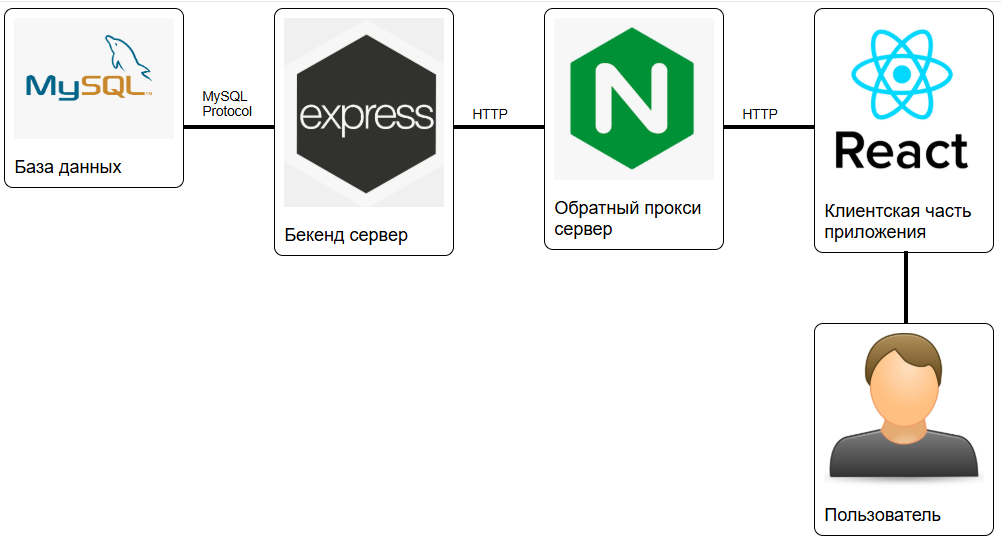
\includegraphics[width=0.5\textwidth]{../images/Схема_веб-приложения.png}
\caption{Рисунок 1}
\end{figure}

Используется следующий стек технологий:

Express JS - бекенд сервер
React JS - фронтэнд часть приложения
MySQL - реляционная база данных
Nginx - обратный прокси сервер

Вкатце опишем для чего нужен каждый элемент смехы:

Бекенд сервер обрабатывает запросы от пользователя, отвечает за аутентификацию, реализует бизнес логику. Например: подобрать рекомендации видео для конкретного пользователя, загрузажать/удалять видео
Фронтэнд - это часть веб-приложения, что находится на стороне пользователя. Пользователь загружает статические файлы сайта,
которые в последующем исполняются в браузере. HTML отвечает за разметку, CSS добавляет стили, а JS отвечает за функциональность - делает сайт живым.
База данных необходима для удобного хранения большого количества данных
Обратный прокси сервер выполняет вспомогательные операции с запросами. Помимо перенаправления запросов, он также может выполнять сжатие, кеширование, предоставлять доступ к файлам
балансировать нагрузку

Характеристи аппаратной части сервера
Все части веб приложения, разумеется кроме клиентской части, находятся на удалённом сервере со следующими характеристиками:

CPU 1 vCPU
RAM 2 GB
Storage 20 GB
Speed 500 Mbps

2.2 Сценарий работы пользователя
Пользователь переходит по ссылке или вводит в строку поиска http://example-videohosting.ru. В этом случае на сервер передаётся HTTP Get запрос, по которому обычно находится index.html файл.
Обычно этот файл выглядит следующим образом:
<!DOCTYPE html>
<html lang="en">
<head>
    <meta charset="UTF-8">
    <meta name="viewport" content="width=device-width, initial-scale=1.0">
    <title>Videohosting</title>
    <link rel="stylesheet" href="./main.css">
    <script src="./main.js"></script>
</head>
<body>
    <img src="./assets/images/image.png">
    ...
</body>
</html>

После загрузки файла браузер начинает его обрабатывать: строится DOM (Document Obejct Model / представление HTML-документа в виде дерева элементов), подгружатся CSS файлы (<link rel="stylesheet" href="./main.css">), подгружаются и исполняются JS файлы, подгружатся и отрисовываются изображения.
Когда этот процесс завершится, можно считать, что приложение полностью загружено и готово к использованию.
Далее пользователь может выполнять HTTP запросы для отправки форм, подзагрузки данных с бекенд сервера.
Статические данные - это данные, которые неизменны для каждого пользователя. К ним можно отнести HTML, JS, CSS файлы сайта и в целом все изображения
Динамические данные - это данные, меняющиеся во время работы приложения. К ним можно отнести информацию о видео (видео могут добавляться/удаляться, изменяется количество просмотров, лайков и т.д)
Мы отдельно рассмотрим сжатие статических и динамических данных.
Дадим краткое описание методов сжатия данных, которые будут использоваться в данной работе
2.3 О форматах изображений
Перед тем как приступить к описанию форматов приведу критерии, по которым я буду их сравнивать:

Степень сжатия - отношение размеров исходного (формат PNG) и сжатого изображений
Скорость компрессии/декомпрессии - как быстро сервер сожмёт изображение и как быстро клиент его разархивирует и отрисует
Совместимость с разными браузерами - важный параметр, так как формат с низким процентом поддреживаемостм не может использоваться в реальном приложении из-за риска потерять большую часть пользователей. Для оценки этого параметра я буду использовать данные с сайта https://caniuse.com/, являющимся де-факто авторитетным справочником о технологиях в браузере.

На сегодняшний день в основном используются шесть форматов:

JPEG
PNG
WebP
AVIF
HEIC
SVG

Поговорим про каждый из них по отдельности
JPEG
Filename extension: jpg jpeg jpe jif jfif jfi
MIME type: image/jpeg
JPEG (Joint Photographic Expert Group) поддерживается всеми браузерами, один из самых популярных форматов изображений.
Поддержииваются изображения с линейным размером не более 65535 x 65536 пикселов.
Алгоритм JPEG наиболее эффективен для сжатия фотографий, содержащих реалистичные сцены с плавными переходами яркости и цвета. Для храненения чертежей, текстовой и знаковой графики лучше использовать PNG, GIF,
либо использовать режим сжатия Lossless JPG.
Уделим этому формату больше внимания чем остальным, так как он зарекомендавал себя временем и применяется много больше других. Позволяет сжимать изображения как с потерями, так и без потерь.
На примере JPEG, мы также постараемся понять, как можно регулировать степень сжатия.
При сжатии изображение преоразуется из цветового пространства $RGB$ в $YC{b}C{r}$. Cтандарт ISO/IEC 10918-1 не регламентирует выбор именно YCbCr, допуская другие виды преобразования.
$Y$ - компонента яркости, $С{B}$, $C{R}$ - синяя и красная цветоразностные компоненты
Преобразование YCbCr можно представить следующими формулами:
$
Y = 0 + (0.299 * R) + (0.587 * G) + (0.114 * B) 
$
$
C_{B} = 128 - (0.168736 * R) - (0.331264 * G) + (0.5 * B)
$
$
C_{R} = 128 + (0.5 * R) - (0.418688 * G) - (0.081312 * B)
$
И обратно:
$
R = Y + 1.402 * (C_{R} - 128)
$
$
G = Y - 0.34414 * (C{B} - 128) - 0.71414 * (C{R} - 128)
$
$
B = Y + 1.772 * (C_{B} - 128)
$
После преобразования $RGB -> YС{B}C{R}$ для каналов $C{B}$, $C{R}$, отвечающих за цвет может выполняться «прореживание», где каждому блоку
из 4 пикселей (2x2) ставится в соответсвие усреднённое значение $C{B}$, $C{R}$ (Схема прореживания 4:2:0). При этом для каждого блока 2x2 вместо 12 значений (4$Y$, 4$C{B}$, 4$C{R}$)
ставится в соответствие 6 значений (4$Y$, $C{B}$, $C{R}$). Если к изображению предъявляются более высокие требования по качеству, могут применяться схемы по сжатия (4:4:0), (4:2:2)
или не применятся вовсе. (4:4:4)
Стандарт допускает прореживание блоков не 22, а 41 или 1*4, но на практике такие схемы применяются довольно редко.
После этого компоненты $Y$, $C_{B}$, $C_{R} разбивается на блоки 8*8. Каждый такой блок подвергается дискретному косинусному преобразованию (ДКП)
Формула для вычисления коэффициентов ДКП $F(u,v)$ блока 8×8:
Коэффициенты ДКП $F(u,v)$ вычисляются по формуле:
$$
F(u,v) = \frac{C(u)C(v)}{4} \sum{x=0}^{7} \sum{y=0}^{7} f(x,y) \cdot \cos\left(\frac{(2x+1)u\pi}{16}\right) \cos\left(\frac{(2y+1)v\pi}{16}\right)
$$
где:

$f(x,y)$ — значение пикселя в позиции $(x,y)$,
$u,v$ — частотные координаты (от 0 до 7),
$C(k)$ — нормировочный коэффициент:
$$
C(k) = \begin{cases}
\frac{1}{\sqrt{2}} & \text{при } k=0, \
1 & \text{иначе}.
\end{cases}
$$

Далее к полученной матрице применяется квантование (зависит от степени сжатия):
$
Q(u, v) = round(\frac{F(u, v)}{Q_{table}(u, v)})
$
После этого многие высокочастотные коэффициенты становятся нулевыми.
Далее полученные коэффициенты записываются в массив и кодируются с помощью кодов Хаффмана.
PNG
Filename extension: png
MIME type: image/png
PNG (Portable Network Graphics) — это растровый формат изображения, который предлагает сжатие без потерь. Еще одна особенность PNG формата — поддержка альфа-канала (прозрачности). Поддерживается всеми браузерами
Согласно сайту caniuse.com поддерживается 92,6% браузеров весной 2025 года.
WebP
Filename extension: webp
MIME type: image/webp
WebP — это формат изображений, разработанный Google, который предлагает сжатие изображений с потерями и без потерь. Он призван обеспечить высокое качество изображений при меньших размерах файлов.
Согласно сайту caniuse.com поддерживается 95,92% браузеров весной 2025 года.
AVIF
AVIF (AV1 Image File Format) — это современный формат изображений, основанный на технологии сжатия AV1. Он предназначен для обеспечения высокого качества изображений при более низком размере файлов. Согласно сайту caniuse.com поддерживается 92,6% браузеров.
Согласно сайту caniuse.com поддерживается 93,71% браузеров весной 2025 года.
HEIF/HEIC
Filename extension: heif heic
MIME type: image/heif image/heic
HEIF (High Efficiency Image Format) — это современный формат изображений, который обеспечивает высокую эффективность сжатия и поддержку различных функций, таких как анимация, HDR, прозрачность и многослойность.
HEIC (High Efficiency Image Container) — это контейнерный формат файла, который используется в том числе и для хранения изображений в формате HEIF, как пример можно привести Live Photos сделанные на iPhone.
Согласно сайту caniuse.com поддерживается 13,99% браузеров весной 2025 года, только устройствами Apple. По причине низкой совместимости в измерениях участвовать не будет. 
SVG
Filename extension: svg
MIME type: image/svg+xml
SVG (Scalable Vector Graphics) — это формат изображений, основанный на XML, который описывает двумерные векторные графики с использованием векторных объектов, таких как линии, кривые, формы и текст. Используется для логотипов и векторных изображений. Для растровых изображений не подходит, поэтому в измерениях участвовать не будет. 
Согласно сайту caniuse.com поддерживается 96,99% браузеров весной 2025 года.
2.4 О алгоритмах сжатия текстовых данных без потерь
Алгоритм Хаффмана
Префиксный код - такой код, ни один символ которого не входит в любой другой
Идея алгоритма состоит в том, что если мы знаем вероятности появления символов, можно описать процедуру построения оптимальных префиксных кодов. Символам с наибольшей вероятностью ставятся в соотвествие более короткие коды.
Алгоритм на входе получает таблицу частотностей символов в сообщении. Далее на основании этой таблицы строится дерево кодирования Хаффмана:

Символы входного алфавита образуют список свободных узлов. Каждый лист имеет вес, который может быть равен либо вероятности, либо количеству вхождений символа в сжимаемое сообщение.
Выбираются два свободных узла дерева с наименьшими весами.
Создается их родитель с весом, равным их суммарному весу.
Родитель добавляется в список свободных узлов, а два его потомка удаляются из этого списка.
Одной дуге, выходящей из родителя, ставится в соответствие бит 1, другой — бит 0. Битовые значения ветвей, исходящих от корня, не зависят от весов потомков.
Шаги, начиная со второго, повторяются до тех пор, пока в списке свободных узлов не останется только один свободный узел. Он и будет считаться корнем дерева.

Построим дерево на конкретном примере, пусть в сообщении имеются символы А, Б, В, Г, Д с частотнастями:

A 15
Б 7
В 6
Г 6
Д 5

\begin{figure}[h!]
\centering
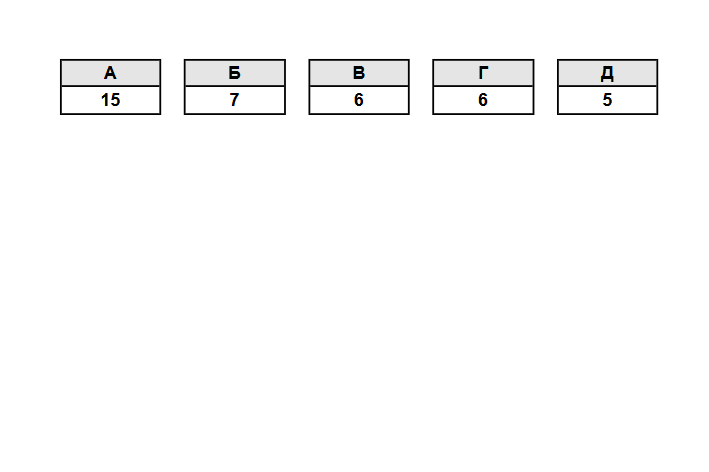
\includegraphics[width=0.5\textwidth]{../images/haffman/phase0.png}
\caption{Рисунок 2}
\end{figure}

\begin{figure}[h!]
\centering
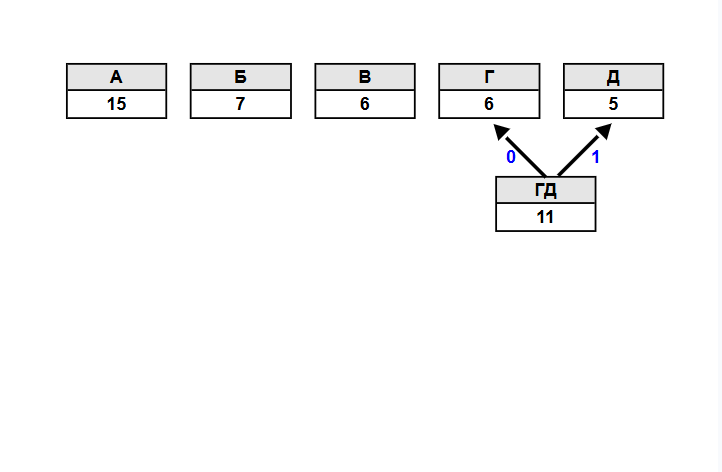
\includegraphics[width=0.5\textwidth]{../images/haffman/phase1.png}
\caption{Рисунок 3}
\end{figure}

\begin{figure}[h!]
\centering
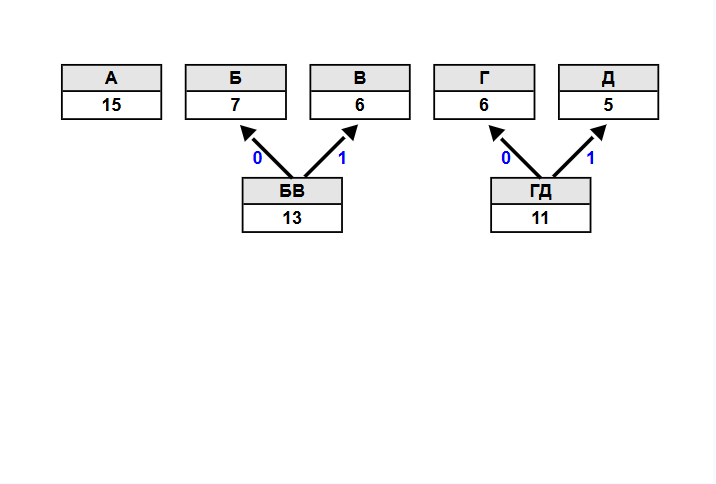
\includegraphics[width=0.5\textwidth]{../images/haffman/phase2.png}
\caption{Рисунок 4}
\end{figure}

\begin{figure}[h!]
\centering
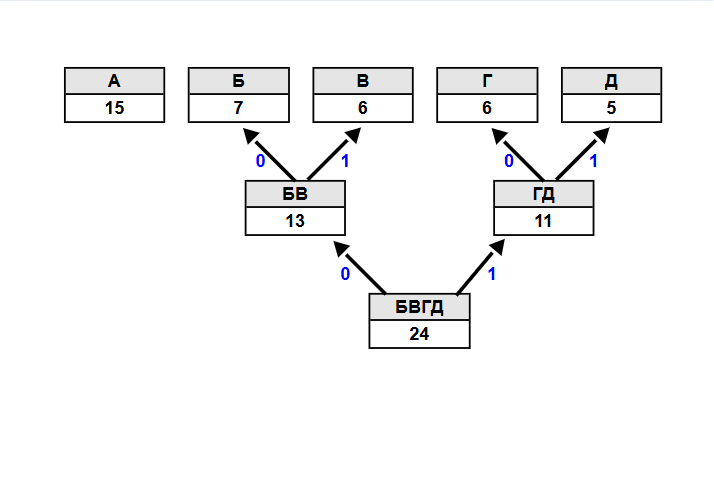
\includegraphics[width=0.5\textwidth]{../images/haffman/phase3.png}
\caption{Рисунок 5}
\end{figure}

\begin{figure}[h!]
\centering
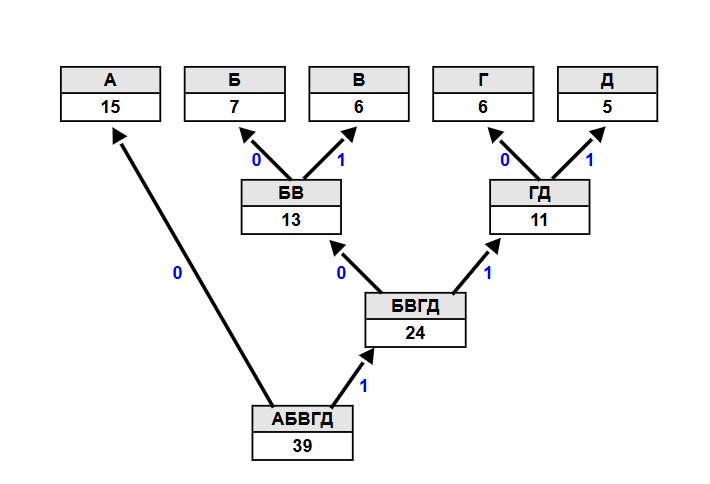
\includegraphics[width=0.5\textwidth]{../images/haffman/phase4.png}
\caption{Рисунок 6}
\end{figure}

В итоге получим следующие префиксные коды:

A 0
Б 100
В 101
Г 110
Д 111

На данный момент, браузером поддерживаются два основных алгоритма метода текстовых файлов (css, html, js):

Gzip
Brotli

Перед тем как приступить к описанию приведённых алгоритмов, следует рассказать о семействе алгоритмов LZ, в частности LZ77, так как оба алгоритма основываются на нём.
Алгоритмы словарного сжатия Зива-Лемпела появились во второй половине 70-х гг. Это были так называемые алгоритмы LZ77 и LZ78, разработанные совместно Зивом (Ziv) и Лемпелом (Lempel). В дальнейшем первоначальные схемы подвергались множественным изменениям, в результате чего мы сегодня имеем десятки достаточно самостоятельных алгоритмов и бессчетное количество модификаций.
LZ77 и LZ78 являются универсальными алгоритмами сжатия, в которых словарь формируется на основании уже обработанной части входного потока, т. е. адаптивно. Принципиальным отличием является лишь способ формирования фраз.
Алгоритм LZ77
Алгоритм LZ77 является родоначальником целого семейства словарных схем - так называемых алгоритмов со скользящим словарем, или скользящим окном. Действительно, в LZ77 в качестве словаря используется блок уже закодированной последовательности. Как правило, по мере выполнения обработки положение этого блока относительно начала последовательности постоянно меняется, словарь "скользит" по входному потоку данных. Скользящее окно имеет длину N, т. е. в него помещается N символов, и состоит из двух частей:

последовательности длины W=N-n уже закодированных символов, которая и является словарем;
упреждающего буфера, или буфера предварительного просмотра (lookahead), длины n; обычно n на порядки меньше W.
Пусть к текущему моменту времени мы уже закодировали t символов, последние W символом будут составлять наш словарь. На каждой итерации алгоритма мы ищем самое длинное вхождение префиксной строки упреждающего буфера, начиная с t+1 символа в словаре + упреждающем буфере, но важно, чтобы часть строки лежала в словаре. Полученная в результате поиска фраза кодируется с помощью двух чисел:


смещения (offset) от начала буфера
длины соответствия, или совпадения
Смещение и длина соответствия играют роль указателя (ссылки), однозначно определяющего фразу. Дополнительно в выходной поток записывается символ s (подумайте зачем), непосредственно следующий за совпавшей строкой буфера.

Что касается декодирования сжатых данных, то оно осуществляется путем простой замены кода на блок символов, состоящий из фразы словаря и явно передаваемого символа. Естественно, декодер должен выполнять Те же действия по изменению окна, что и кодер. Фраза словаря элементарно опре- деляется по смещению и длине, поэтому важным свойством LZ77 и прочих алгоритмов со скользящим окном является очень быстрая работа декодера.
Алгоритм декодирования может иметь следующий вид:
Алгоритмы со скользящим окном характеризуются сильной несимметричностью по времени - кодирование значительно медленнее декодирования, поскольку при сжатии много времени тратится на поиск фраз.
Формат Deflate
Формат словарного сжатия Deflate, предложенный Кацем (Katz), используется популярным архиватором GZIP. Сжатие осуществляется с помощью алгоритма типа LZH, иначе говоря, указатели и литералы кодируются по методу Хаффмана. Формат специфицирует только работу декодера, т. е. определяет алгоритм декодирования, и не налагает серьезных ограничений на реализацию кодера. В принципе в качестве алгоритма сжатия может применяться любой работающий со скользящим окном, лишь бы он исходил из стандартной процедуры обновления словаря для алгоритмов семейства LZ77 и использовал задаваемые форматом типы кодов Хаффмана
Закодированные в соответствии с форматом Deflate данные представляют собой набор блоков, порядок которых совпадает с последовательностью соответствующих блоков исходных данных. Используется 3 типа блоков закодированных данных:

состоящие из несжатых данных;
использующие фиксированные коды Хаффмана;
использующие динамические коды Хаффмана.
Длина блоков первого типа не может превышать 64 Кб, относительно других ограничений по размеру нет. Каждый блок типа 2 и 3 состоит из двух частей:


описания двух таблиц кодов Хаффмана, использованных для кодирования данных блока;
собственно закодированных данных.
Коды Хаффмана каждого блока не зависят от использованных в предыдущих блоках. Cамо описание динамически создаваемых кодов Хаффмана является, в свою очередь, также сжатым с помощью фиксированных кодов Хаффмана, таблица которых задается форматом.
Алгоритм словарного сжатия может использовать в качестве словаря часть предыдущего блока (блоков), но величина смещения не может быть больше 32 Кб. Данные в компактном представлении состоят из кодов элементов двух типов:
литералов (одиночных символов);
указателей имеющихся в словаре фраз; указатели состоят из пары <длина совпадения, смещение>

Длина совпавшей строки не может превышать 258 байт, а смещение фразы - 32 Кб. Литералы и длины совпадения кодируются с помощью одной таблицы кодов Хаффмана, а для смещений используется другая таблица; иначе говоря, литералы и длины совпадения образуют один алфавит. Именно эти таблицы кодов и передаются в начале блока третьего типа.
Алгоритм декодирования Deflate
Сжатые данные декодируются по следующему алгоритму:
TODO
Алгоритм словарного сжатия для DEFLATE
Как уже указывалось, формат Deflate не имеет четкой спецификации алгоритма словарного сжатия. Разработчики могут использовать какие-то свои алгоритмы, подходящие для решения специфических задач.
В качестве примера приведу свободный от патентов алгоритм сжатия для Deflate, используемый в разрабатываемой Info-ZIP group утилите Zip.
Формат сжатия Gzip (GNU zip)
Это утилита для сжатия и распаковки файлов, которая широко используется в UNIX-системах.
Формат файла gzip состоит из 3 основных частей:

Заголовок: Содержит информацию о типе файла, имени оригинального файла, времени создания, уровне сжатия и других параметрах.
Тело: Содержит сжатые данные, выполненные с помощью алгоритма DEFLATE.
Контрольная сумма (CRC-32) и Размер оригинала: Эти данные предоставляют возможность проверки целостности и правильности распаковки данных.

Заголовок файла содержит следующие ключевые поля:

ID1 и ID2: Идентификаторы, указывающие на формат gzip (значения - 0x1F и 0x8B).
CM: Метод сжатия (в gzip используется значение 8 для DEFLATE). *
FLG: Биты флагов, которые указывают наличие дополнительных полей и информации.
MTIME: Время последней модификации оригинального файла.
XFL: Дополнительная информация о методе компрессии.
OS: Платформа, на которой был создан/сжат файл (gzip).

Другие значения для этого поля теоретически могут быть использованы для обозначения различных методов сжатия, но сам формат gzip и его стандартная реализация подразумевают использование только DEFLATE. На практике, если gzip файл содержит метод сжатия, отличный от DEFLATE, стандартные утилиты для работы с gzip файлами могут его не поддерживать и не распознать.
За счёт чего можно добиться разных степеней сжатия?
Т.к формат Deflate не имеет четкой спецификации алгоритма словарного сжатия, разработчики могут использовать различные модификации LZH, подбирая параметры для обеспечения желаемого соотношения скорости и коэффициента сжатия.
В приведённом примере алгоритма сжатия DEFLATE, можно менять match_len(t+1) = L
2.5 Инструменты разработчика браузера
Браузеры и JavaScript
На сегодняшний день существует два вида браузеров:

Основанные на движке Chromium V8 от Google (https://github.com/v8/v8) такие, как Gooogle Chrome, Yandex Browser, Microsoft Edge и другие
Firefox, использующий Quantum

Дело в том, что JavaScript, использующийся в веб приложениях, - скриптованный язык, существует спецификация ESMA Script (https://262.ecma-international.org/), в которой написано, что должен делать язык, но реализация не указана. Реализация фукнций языка ложится на разработчиков браузеров. Здесь, в отличие от Си или Java, не существует компиляторов или Java Virtual Machine. Разрабочики веб-приложений точно не знают, что происходит "под капотом".
Для получения информации о времени выполнения, скорости загрузки, использования памяти можно использовать инструменты разработчика (DevTools). Её можно открыть в любом браузере, нажав F12
Какие функции предоставляет консоль разработчика
Реализации DevTools отличаются в зависимости от браузера. Но в целом, DevTools у браузеров на Chromium очень похожи.
Я буду брать примеры из Google Chrome
Нас интересуют две вкладки:
Networks
\begin{figure}[h!]
\centering
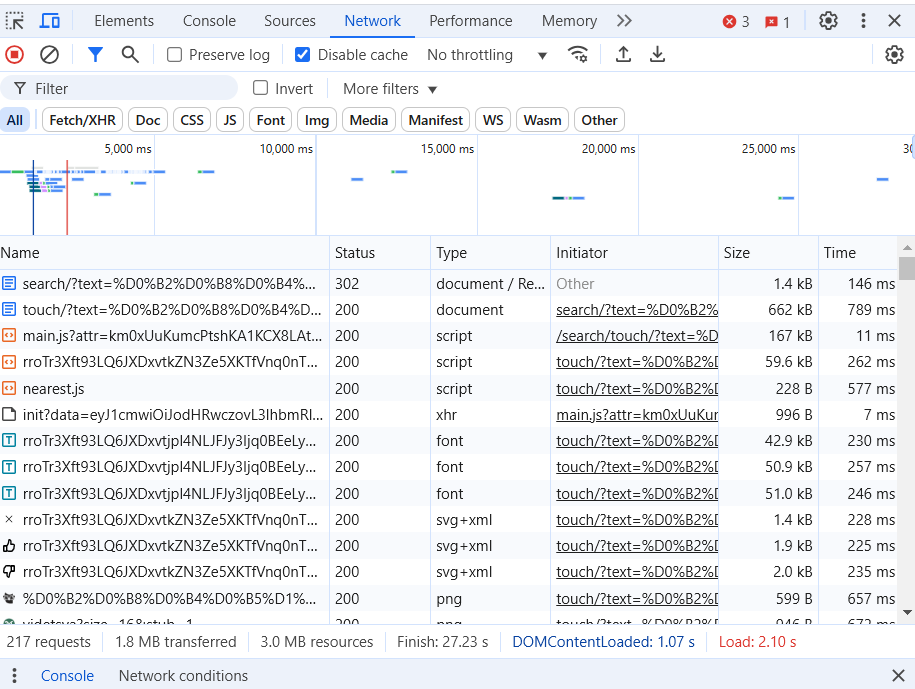
\includegraphics[width=0.5\textwidth]{../images/network.png}
\caption{Рисунок 7}
\end{figure}

На этой вкладке можно посмотреть все сетевые запросы, выполненные браузером на данной странице, узнать статус запроса, тип, размер ответа и общее время, потраченное на HTTP запрос,
\begin{figure}[h!]
\centering
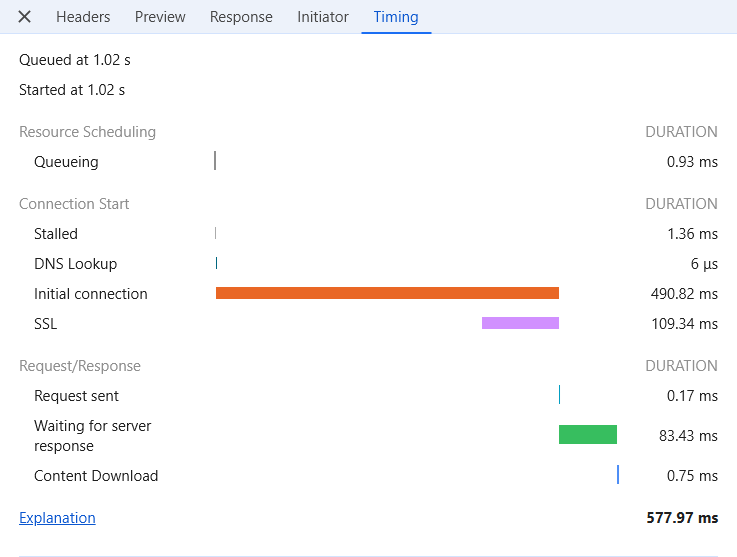
\includegraphics[width=0.5\textwidth]{../images/network__timing.png}
\caption{Рисунок 8}
\end{figure}

Если нажать на конкретный запрос, можно будет узнать такие параметры, как

Время, когда запрос был отправлен (время отсчитывается от момента перехода на сайт)
Queueing Очередь . Браузер ставит запросы в очередь перед началом соединения и когда:
Есть запросы с более высоким приоритетом. Приоритет запроса определяется такими факторами, как тип ресурса, а также его расположение в документе.
Для этого источника уже открыто шесть TCP-соединений, что является пределом. (Применимо только к HTTP/1.0 и HTTP/1.1.)
Браузер ненадолго выделяет место в дисковом кеше.
Stalled Запрос мог быть остановлен после начала соединения по любой из причин, описанных в Queueing
Initial connection. Временные затраты на TSL/SSL handshake, если используется HTTPs, на TCP Handshake
Время, затраченное, на отправку запроса
Время ожидание ответа от сервера
Сколько времени затрачено на загрузку содержимого запроса

Суммарное время запроса складывается из всех перечисленных отрезков времени
Как можно заметить, по этим параметрам не удаётся опеределить время, затраченное на декодирование запроса
Немного о HTTP
Считаю уместным сказать несколько слов о HTTP протоколе, чтобы иметь лучшее представление, о том, как с технической точки зрения применяется сжатие.
Первым делом браузер осуществляет HTTP запрос, прикрепляя заговок Accept-encoding. Современные браузеры поддерживают Gzip, Deflate, Brotli, Zstandard, и заголовок выглядит следующим 
образом: Accept-encoding: gzip, deflate, br, zstd. Сервер обрабатывает запрос, применяя к телу HTTP запроса один из алгоритмов, указанных в Accept-encoding. В ответе сервер прикрепляет заголовок Content-encoding, например Сontent-encoding: br, говорящий о применённом алгоритме. Браузер получив ответ, может продолжить загрузку тела HTTP запроса. 
Performance
\begin{figure}[h!]
\centering
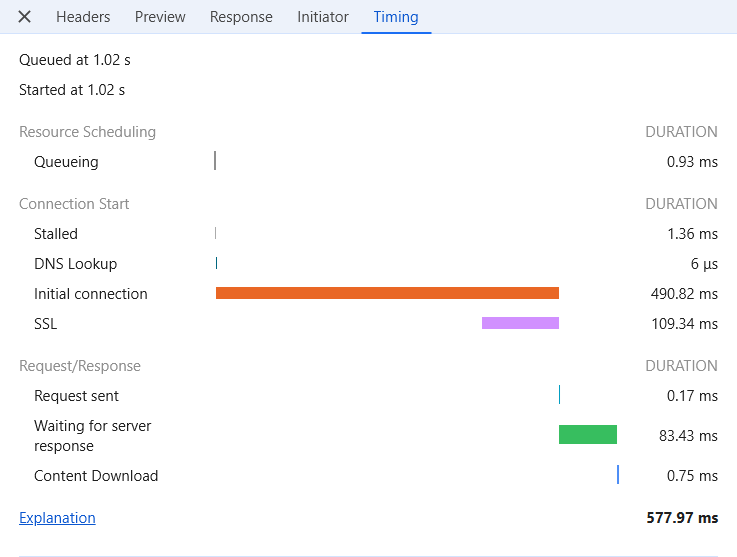
\includegraphics[width=0.5\textwidth]{../images/network__timing.png}
\caption{Рисунок 9}
\end{figure}

Largest Contentful Paint (LCP) (https://web.dev/articles/lcp) сообщает о времени рендеринга самого большого изображения, текстового блока или видео,
видимого в окне просмотра, по отношению к моменту, когда пользователь впервые перешёл на страницу. Браузер измереяет это время, как момент, когда построится DOM дерево, исполнится JavaScript код, применятся CSS стили, загрузятся и отрисуются изображения. Этот показатель используется поисковиками для ранжирования сайтов: чем ниже $T_{LCP}$, тем выше сайт в выдаче.
Поэтому я буду обращать особое внимание LCP.
На этой вкладке мы так же можем применить замедление к процессору или к сети
Для сети существует несколько режимов:
2. Low-end Mobile (регламентировано для 3G):

Скорость загрузки (Download): 400 Kbps.
Скорость отправки (Upload): 400 Kbps.
Задержка (Latency): ~400 мс.

3. Regular 3G

Скорость загрузки (Download): 750 Kbps.
Скорость отправки (Upload): 250 Kbps.
Задержка (Latency): ~100 мс.

4. Good 3G

Скорость загрузки (Download): 1.5 Mbps.
Скорость отправки (Upload): 750 Kbps.
Задержка (Latency): ~40 мс.

Можно настроить и свою конфигурацию
Замедление процессора
CPU throttling в DevTools используется для замедления работы процессора в целях эмуляции менее мощных устройств или реальных условий работы пользователей.
Это особенно полезно для тестирования производительности, чтобы понять, как сайт или приложение будет работать на слабых устройствах,
таких как смартфоны, или в условиях высокой нагрузки.
Из моих наблюдений
 Тротлинг в DevTools реализован программно. Браузер замедляет выполнение базовых функций JavaScript (sort, map, for) в указанное число раз (4x, 6x, 20x).
Исходя из этого, можно предположить, что замедление CPU не отразиться на времени, затраченное на декодирование файлов

Также можно замерить, какое замедление процессора нужно применить для эмуляции мобильных устройств. На моём компьютере это оказалось от 2x (для среднего сегмента смартфонов) и 6x (для low сегмента).
3. Измерения и анализ полученных результатов
3.1 Сравнение форматов изображений
Изначально все изображения в png
Конвертация из PNG в JPEG с качеством 0.8 - обеспечивающее баланс между качеством и степенью сжатия, из PNG в WebP на сайте https://image.online-convert.com/convert/
Из PNG в Avif на сайте https://converter.app/png-to-avif
Из PNG в Heic на сайте https://png2heic.com/
Выбраны 10 различных изображений (людей, природы, котов) в формате PNG и сконвертированы в JPG, Webp, Avif и Heic
\begin{figure}[h!]
\centering
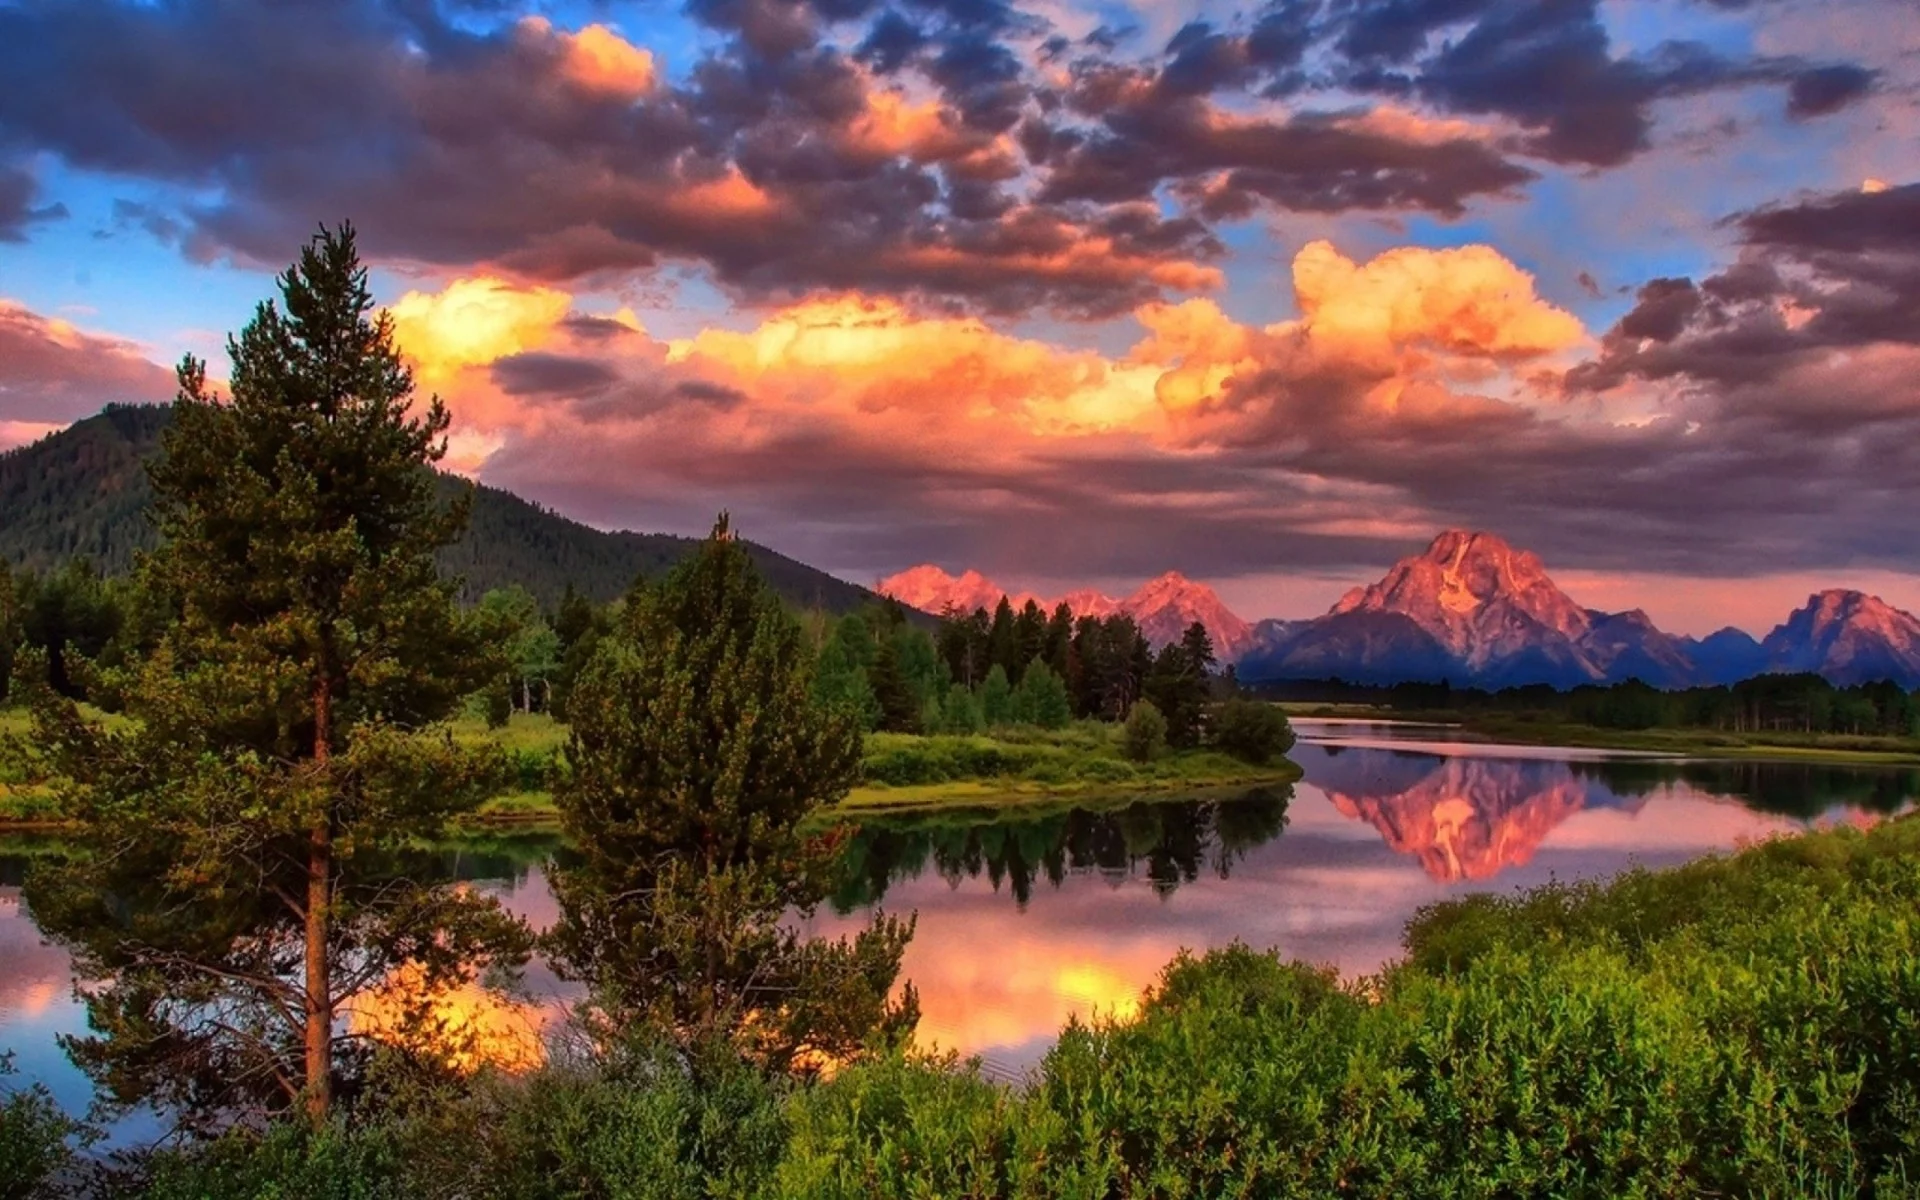
\includegraphics[width=0.5\textwidth]{../images/image_comp/image1.png}
\caption{Рисунок 10}
\end{figure}

\begin{figure}[h!]
\centering

\includegraphics[width=0.5\textwidth]{../images/image_comp/image4.png}
\caption{Рисунок 11}
\end{figure}

Вес 10-ти изображений в форматах:

PNG 18,0 Мб
JPEG 1,66 Мб
WebP 1,42 Мб
Avif 1,00 Мб
Heic 1,04 Мб

Измерение времени декодирования
Я начал с того, что попытался получить информацию о времени декодирования напрямую из DevTools. Для формата JPEG получилась следующая картина:
\begin{figure}[h!]
\centering
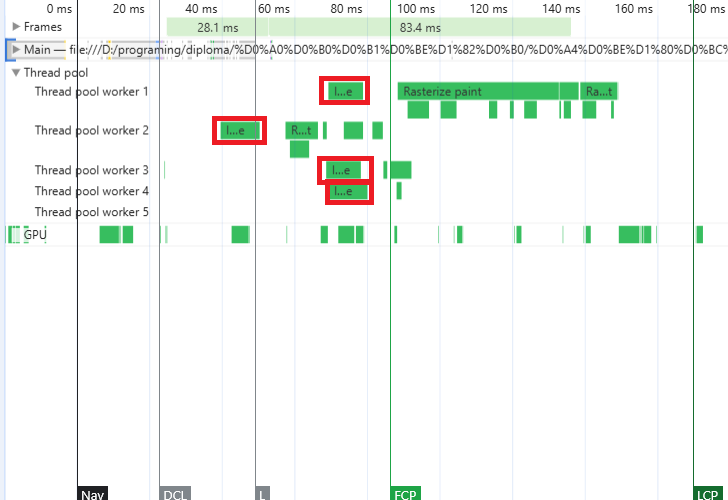
\includegraphics[width=0.5\textwidth]{../images/image_comp/devtools.png}
\caption{Рисунок 12}
\end{figure}

На данной диграмме мы видим временные интервалы соответствующие декодированию и растеризации изображений.
По оси X отложено время в милисекундах, по оси Y представлены задействованные потоки процессора
Как можно заметить, браузер умеет декодировать изображения параллельно.
В основном реализуется следующах схема:

Браузер скачивает файл
Декодирует
Растеризует

Но, т.к JPEG поддерживает последовательное декодирование, может получится так, что браузер сначала декодирует часть изображения,
растеризует декодированную часть, декодирует ещё одну часть и так далее. На практике я наблюдал разбиение изображения на три части
Для изображения весом 344kB я получил время декодирования: $T{dec}=13,4 \pm 1,08мс$, время расторизации: $T{ras}=8,9 \pm 0,91мс$
Дела обстаят хуже с другими форматами. Браузер не даёт информации о времени декодирования.
Для avif:
\begin{figure}[h!]
\centering
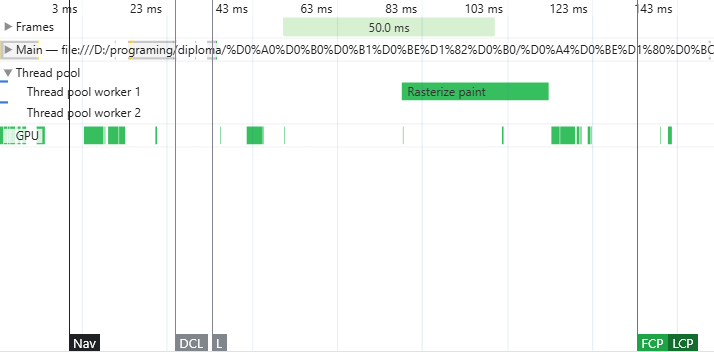
\includegraphics[width=0.5\textwidth]{../images/image_comp/avif_one_image.png}
\caption{Рисунок 13}
\end{figure}

Время расторизации для avif $T_{ras}=34,9 \pm 3,21мс$, что заметно хуже чем у JPG
Мы можем измерить время, потраченное на декодирование + расторизацию косвенно. Предположим, что LCP измеряется по следующей формуле
$
T{LCP} = T{проч} + T{down} + T{dec+ras}
$
где

$T_{проч}$ - время на рендеринг DOM, время на отправку запроса HTTP и прочие функции браузера, которые не зависят от формата
$T{down}$ - время на загрузку файла, для JPEG $T{down} = 1,3 \pm 0,2 мс$, для PNG $T_{down} = 2,4 \pm 0,3 мс$. Этим можно пренебречь
$T_{dec+ras}$ - время на декодирование и растеризацию

Тогда замерив LCP для разных форматов, можно найти разность $T_{dec+ras}$.
Результаты для LCP следующие:
\begin{table}[h!]
\centering
\caption{Таблица 1}
\begin{tabular}{|c|c|c|}
\hline
Формат & $\overline{LCP}$, мс & $\sigma$, мс \\
\hline
JPEG & 73,5 & 8,05 \\
\hline
PNG & 141,3 & 7,51 \\
\hline
AVIF & 139,5 & 6,6 \\
\hline
WebP & 125,3 & 6,51 \\
\hline
\end{tabular}
\end{table}

Считая, что для JPEG $T{dec+ras} = 22,8 \pm 2мс$. JPEG $T{dec+ras}$:
\begin{table}[h!]
\centering
\caption{Таблица 2}
\begin{tabular}{|c|c|c|}
\hline
Формат & $\overline{LCP}$, мс & $\sigma$, мс \\
\hline
JPEG & 22,8 & 2 \\
\hline
PNG & 90,6 & 9,51 \\
\hline
AVIF & 88,8 & 8,6 \\
\hline
WebP & 74,6 & 8,51 \\
\hline
\end{tabular}
\end{table}

Проанализуем полученные результаты. Самыми лучшими с точки зрения уровня сжатия оказались фотматы HEIС и AVIF.
Тест на 10-ти изображениях показал степень сжатия 18 по сравнению с изначальным форматом PNG.
Наилучшее время декодирования и растеризации достиг формат JPEG. Стоит отметить, что формат PNG, вероятнее всего, оказался худшим по этому показателю не из-за сложности алгоритма декодирования, а из-за байтового размера файла. Компьютеру сложнее обработать большой массив бит. Похожий результат мы увидим в главе, посвещённой статических файлов без потерь
Так как у нас не оказалось однозначного лидера по обоим показателям, попроруем определить критерии оптимального формата с точки зрения LCP. Предположим, у нас есть некоторое изображение.
Также у нас постоянные характеристики аппартой части клиента. Тогда $T{LCP}$ зависит только от двух параметров: $V{down}$ и $i_{comp}$, где:

$V_{down}$ - скорость загрузки пользователя
$i_{comp}$ - формат кодирования

Тогда:
$
T{LCP} = T{LCP}(V{down}, i{comp}) = T^{i}{проч} + T^{i}{down} + T^{i}{dec+ras} = T{проч} + \frac{M{исх}}{k{i}*V{down}} + T^{i}{dec+ras}
$
Используя эту формулу, найдём скорость загрузки пользователя, при которой $T^{JPEG}{LCP} = T^{AVIF}{LCP}$ для протестированного изображания:
$
T{проч} + \frac{M{исх}}{k{JPEG}*V^{equal}{down}} + T^{JPEG}{dec+ras} = T{проч} + \frac{M{исх}}{k{AVIF}*V^{equal}{down}} + T^{AVIF}{dec+ras}
$
$
\frac{M{исх}}{k{JPEG}V^{equal}_{down}} + T^{JPEG}_{dec+ras} = \frac{M_{исх}}{k_{AVIF}V^{equal}{down}} + T^{AVIF}{dec+ras}
$
$
\frac{M{исх}}{k{JPEG}V^{equal}_{down}} - \frac{M_{исх}}{k_{AVIF}V^{equal}{down}}  = T^{AVIF}{dec+ras} - T^{JPEG}_{dec+ras}
$
$
V^{equal}{down} = \frac{M{исх}(k{AVIF}-k{JPEG})}{k{JPEG}k{AVIF}(T^{AVIF}{dec+ras} - T^{JPEG}{dec+ras})}
$
$М{исх} = 2,9$Мб, $k{JPEG} = 8,89$, $k_{AVIF} = 16,14$
$
V^{equal}_{down} = 17,76 мбит/c
$
Что вдвое быстрее хорошего 4G. Выше этой скорости будет эффективнее JPEG, ниже этой скорости - AVIF
Чтобы проверить результаты расчётов, предлагаю сравнить $T_{LCP}$ у JPEG и AVIF для разных скоростей:

Fast 4G 7,5 мбит
«Doble» 4G 18 мбит/c
Без замедления

\begin{table}[h!]
\centering
\caption{Таблица 3}
\begin{tabular}{|c|c|c|}
\hline
Формат & $\overline{LCP}$, мс & $\sigma$, мс \\
\hline
Fast 4G, JPEG & 799,83 & 20,55 \\
\hline
Fast 4G, AVIF & 736,51 & 13,30 \\
\hline
«Doble» 4G JPEG & 689,07 & 23,28 \\
\hline
«Doble» 4G AVIF & 689,65 & 15,64 \\
\hline
Без замедления JPEG & 151,82 & 5,96 \\
\hline
Без замедления AVIF & 198,39 & 25,97 \\
\hline
\end{tabular}
\end{table}

Измерения подтверждают выведенную формулу. Может возникнуть вопрос, почему в этом измерении без замедления $LCP$ оказался больше чем в предыдущем опыте.
Дело в том, был использован сервер раздачи статических файлов, что позволило конфигурировать параметры сети. Также стоит подметить, что LCP увелился в случаях 4G и Doble 4G из-за искусстевенной задержки ответа сервера, что эмулирует реальную 4G сеть.
Практические рекомендации
Учитывая, что полученная $V^{equal}_{down} = 17,76 мбит/c$ соответсвует пограничной скорости мобильного интернета, следует использовать формат AVIF, если целевая аудитория сайта - пользователи мобильных устройств, и JPEG, если используются десктопные устройства (100мбит/c). Конечно, в случае, когда нам не требуется поддержка прозрачности. В противном случае рекомендую использовать WebP. 
Случай с множеством изображений
Когда на сайте несколько изображений, следует учитывать возможность параллельного декодирования и растеризации, в этом случае $V^{equal}_{down}$ будет другой. Формула расчёта зависит от числа потоков, задействованных браузером.
3.2 Сжатие статических файлов браузера с помощью Gzip, Brotli
Что измеряем
Для алгоритмов gzip, brotli будут измерены

Степень сжатия
Время сжатия
Время декомпрессии

В качестве исходных данным будут использованы минифицированные версии трёх веб-приложений:

Dating App (DA)
Videohosting (VH)
Angular conduit (AC)

Технические характеристики устройства
Процессор: Intel(R) Core(TM) i5-10210U CPU @ 1.60GHz 2.11 GHz
Оперативная память: 8,00 ГБ
Операционная система: Windowws 11, версия 24H2, WSL Linux Ubuntu 20.04
Условия проведения эксперимента, обработка данных
Для сжатия использована утилита gzipper (https://www.npmjs.com/package/gzipper) на node.js
Для декопрессии использованы утилиты gunzip, brotli на Linux
Для замеров времени декомпрессии использован hyperfine
При измерении скорости для каждой точки было проведено 20 измерений и применён метод усечённого среднего (10%)
Так же построены минимумы по времени
Для точности измерений были отключены фоновые процессы операционной системы
В веб-приложениях были удалены файлы с изображениями, т.к они уже сжаты с помощью специальных алгортмов для изображений (jpg, webp, avif)
Изначальный размер
Изначальный размер приложений:

Dating App (DA) 999КБ
Videohosting (VH) 479КБ
Angular conduit (AC) 456КБ

Измерение степени сжатия
Для Gzip
\begin{figure}[h!]
\centering
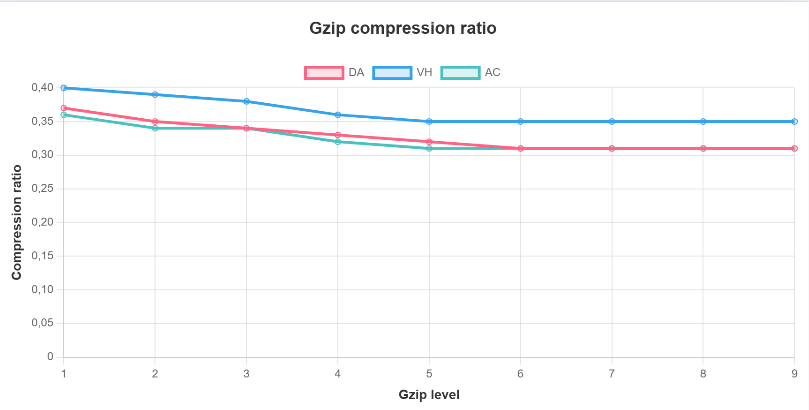
\includegraphics[width=0.5\textwidth]{../images/gzip_compress_ratio.png}
\caption{Рисунок 14}
\end{figure}

для Brotli
\begin{figure}[h!]
\centering
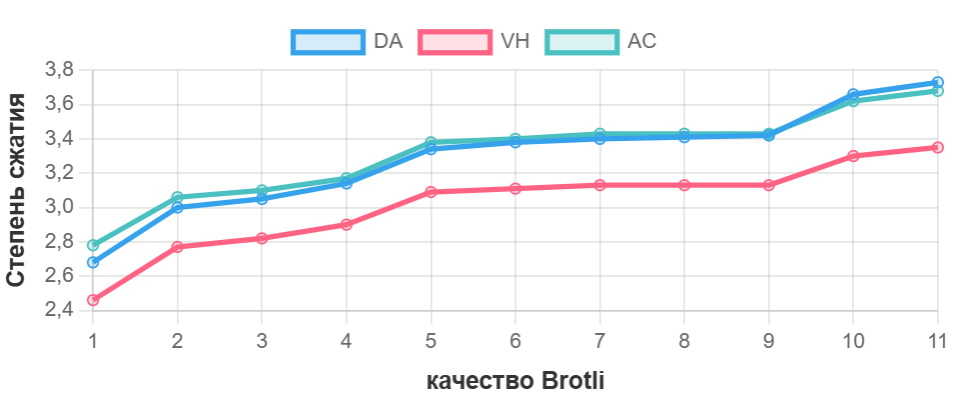
\includegraphics[width=0.5\textwidth]{../images/brotli_compressed_ratio.png}
\caption{Рисунок 15}
\end{figure}

Измерение времени сжатия
Для Gzip
\begin{figure}[h!]
\centering
\includegraphics[width=0.5\textwidth]{../images/Gzip\ compression\ time\ (Trimmed\ Mean).png}
\caption{Рисунок 16}
\end{figure}

Для Brotli
\begin{figure}[h!]
\centering
\includegraphics[width=0.5\textwidth]{../images/Brotli\ compression\ time\ (Trimmed\ Mean).png}
\caption{Рисунок 17}
\end{figure}

Также построены графики минимального времени для странение влияния случайных факторов:

При замерах производительности система может испытывать фоновые процессы (ОС, другие программы, прерывания, кэш-CPU).
Минимальное время показывает, как быстро программа работает в идеальных условиях (без помех).

Для Gzip
\begin{figure}[h!]
\centering
\includegraphics[width=0.5\textwidth]{../images/Gzip\ compression\ time\ (min).png}
\caption{Рисунок 18}
\end{figure}

Для Brotli
\begin{figure}[h!]
\centering
\includegraphics[width=0.5\textwidth]{../images/Brotli\ compression\ time\ (min).png}
\caption{Рисунок 19}
\end{figure}

Было замечено, что gzipper тратит 160ms на пустой файл, вероятно это время требуется, чтобы запустить процесс, выделить память. Поэтому также построены графики за вычетом времени на накладные расходы
Для Gzip
\begin{figure}[h!]
\centering
\includegraphics[width=0.5\textwidth]{../images/Gzip\ compression\ time\ (min-overhead).png}
\caption{Рисунок 20}
\end{figure}

Для Brotli
\begin{figure}[h!]
\centering
\includegraphics[width=0.5\textwidth]{../images/Brotli\ compression\ time\ (min-overhead).png}
\caption{Рисунок 21}
\end{figure}

Измерение времени декомпрессии
Измерения времени декомпрессии программой gunzip произведены на Ubuntu Linux 24.04. Для замеров использована утилита hyperfine.
\begin{figure}[h!]
\centering
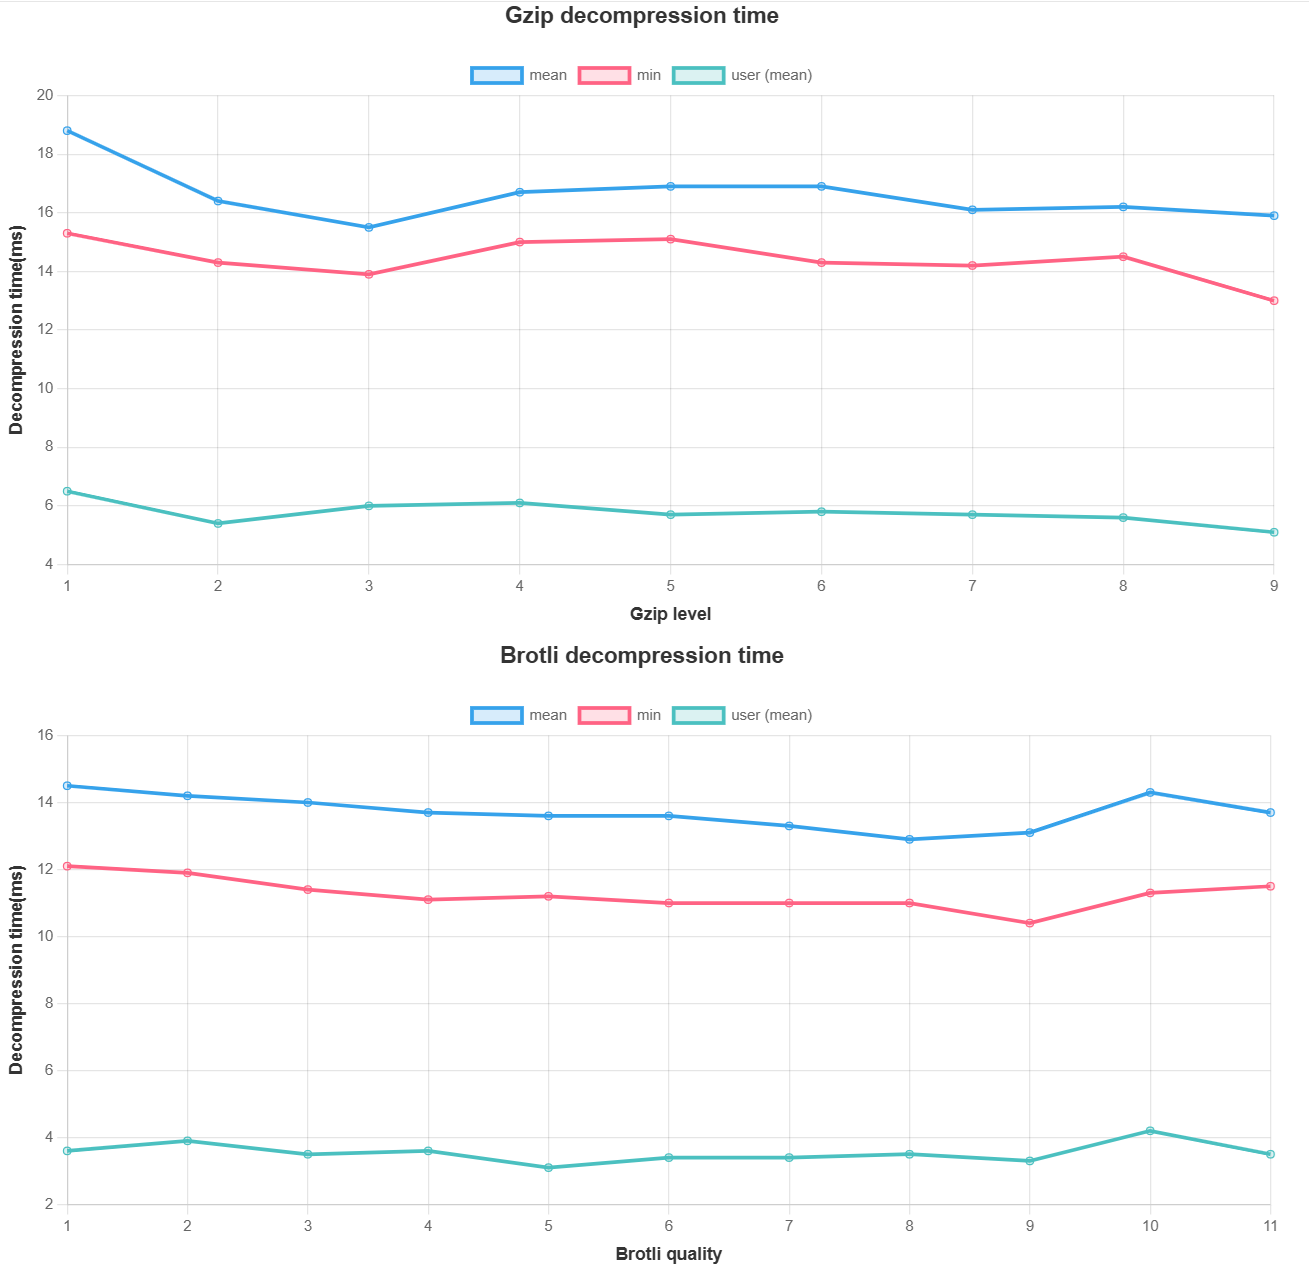
\includegraphics[width=0.5\textwidth]{../images/Decompression_time.png}
\caption{Рисунок 22}
\end{figure}

Как видно, скорость декомпрессии почти не зависит от степени сжатия.
Так же видно, что в среднем brotli быстрее разжимает файлы чем gzip (имеются в виду конкретные программы)
3.3 Реальные замеры сжатия статических файлов в браузере
Постановка эксперимента
В файле со сравнением gzip и brotli, я сжимал самый большой файл проекта Dating App. 765кб -> 193кб.
Сделаем так:
загружаем файл main.js, далее выполняем запрос (fetch). Будем измерять время отправления запроса.
  <body>
    <script src="http://localhost:88/main.js" />
    <script>
      fetch("http://localhost:88/test");
    </script>
  </body>

Как происходит загрузка сайта в браузере:

Загружаем html документ
Парсим html документ
Встречаем <script src="http://localhost:88/main.js" />, что говорит нам: загрузи и исполни скрипт с адреса "http://localhost:88/main.js",
дальше не пойдём, пока этот скрипт не загрузится. В это время как раз входит время, необходимое на скачивание декодирование.
Скрипт я закомментировал, чтобы не испортить измерения сторонними вычислениями.
Дальше выполняем запрос на "http://localhost:88/test". Это служит в качестве маркера. Время отправки запроса мы и будем измерять.

Буду проводить замеры:
Network throttling, CPU throttling

No Throttling, No Throttling (Неограниченная скорость интеренета, мощный процессор)
fast 4g, No Throttling (Быстрый интернет, мощный процессор)
No Throttling, 6x Throttling

Сравню найду время отправки запроса для сжатия brottli 11x и для файла без сжатия. В теории для 3-го случая может получится, что без сжатия будет быстрее,
так как не потребуется тратить время на декодировние.
Но т.к есть подозрения, что CPU throttling не влияет на время декодирования, проведу замеры на своём мобильном телефоне Xiaomi 9T PRO в локальной сети Wi-Fi (300 Mb/s).
Так же дополнительно отключил кеширование на стороне клиента с помощью заголовков "Cache-Control", "Pragma"
Как и в прошлый раз ограничиваю фоновые процессы. 20 замеров на каждую характеристику
Время test запроса в случае с телефоном измерялось на стороне сервера.

$T_{gzip9}=65,35$мс, $\sigma = 9,21$мс
$T_{no comress}=145,10$мс, $\sigma = 34,34$мс

Вывод по статическим файлам JS, CSS, HTML
Результаты измерений показали, что для статических файлов во всех случаях сжатия файлов либо существенно уменьшает время отклика, либо не увеличивает его.
То есть для любых устройств и любых параметров сети сжатие статических файлов будет предпочтительно, причём следует выбирать максимальную степень сжатия будь то gzip 9 или brotli 11
На данном этапе мы разобрались со статическими файлами. Теперь перейдём к динамическим данным, меняющимся с течением времени. Основное отличие состоит в том, что мы не можем сжать данные заранее, приходится применять сжатие "на лету". Наша задача на данном этапе выяснить, как сжатие влияет на такие показатели, как: 
- Количество запросов в секунду (RPS)
- Нагрузка на сеть
- Время ожидание ответа от сервера 
- Время загрузки содержимого запроса
- Общее время запроса
3.4 Нагрузочное тестирование REST запросов (динамические данные)
Описание аппаратной части сервера
Технические характеристики сервера:

CPU 1 vCPU
RAM 2 GB
Storage 20 GB
Speed 1200 Mbps

Технические характеристика моего ноутбука:

CPU 4 ядра
RAM 8 GB
Speed 50 Mbps

В качестве REST сервера используется Node.js express.js, обратный прокси сервер (сжатие http) Nginx
Логика следующая:

клиент заходит на сайт
скачивает статические файлы
когда выполнится js код, выполнится get запрос на получение всех видео /videos/getAll
сервер сделает запрос в базу данных
возвращает ответ

Тестрирование проводится с помощью k6. Замеряются такие параметры, как:

Загрузка ЦП сервера
Использование оперативной памяти сервера
Время ожидание ответа от сервера 
Время загрузки содержимого запроса
Процент успешно выполненных HTTP запросов 

В зависимости от количества запросов в секунду (RPS)
Ответ от сервера представляет собой массив JSON:
[
  {
    title: "Steel Horizon",
    description:
      '"Steel Horizon" is a captivating cinematic journey that explores the boundaries of imagination and reality. With stunning visuals and a compelling narrative, it draws viewers into a richly woven tale full of emotion, suspense, and intrigue. As the characters navigate through complex challenges, deep personal struggles, and unexpected twists, the story unfolds with intensity and grace. Crafted by visionary creators, the film blends elements of classic storytelling with modern cinematic techniques to create an unforgettable experience. Whether you\'re drawn to heartfelt drama, thrilling action, or thought-provoking ideas, this film offers a powerful reflection on humanity, resilience, and discovery.',
    number: 19,
    src_url: "https://cdn.example.com/videos/video_19.mp4",
    preview_url: "/previews/bearwolf.mp4",
    image_url: "/images/bearwolf2.jpg",
    studios: ["MegaPix"],
    tags: ["documentary", "action", "comedy"],
  },
  ...
]

Физический смысл выбранной нагрузки
\begin{figure}[h!]
\centering
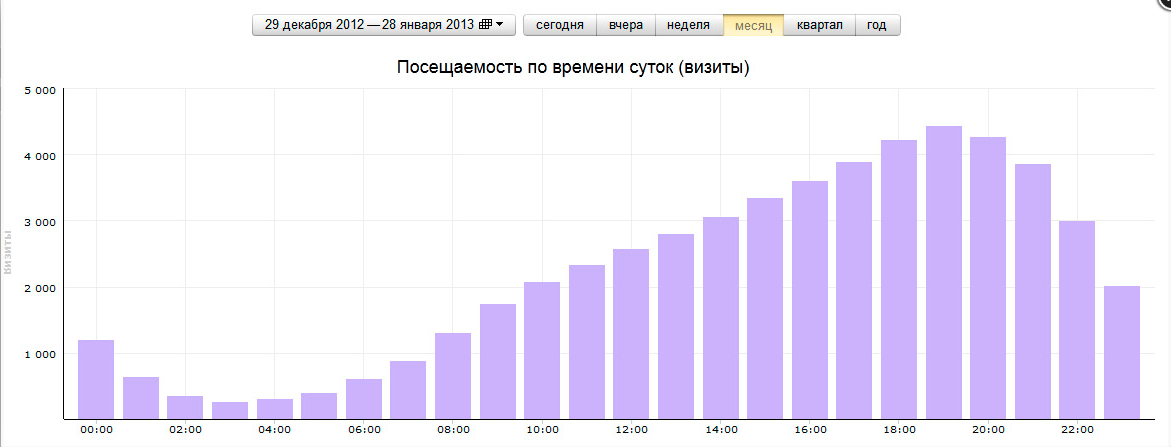
\includegraphics[width=0.5\textwidth]{../images/pedsovet.png}
\caption{Рисунок 23}
\end{figure}

Перед вами статистика посещаемости некоторого сайта за день. Собрано количество посещений за каждый час и построена гистограмма.
Можно заметить неравномерность визитов в течение дня. Так в период с 18:00 до 19:00 количество посещений составило в районе 4000, а с 2:00 до 3:00 менее 500. Это связано с территориальной распределённостью пользователей. Если сайт русскоязычный, то логично предположить, что пик будет приходится на вечернее время по Москве, так как население России преимущественно находится в её европейской части. Поэтому важно узнать, как ведёт себя сервер при разной нагрузке. 
Было проведено два эксперимента соответствующие пиковой и умеренной нагрузке. Предполагается, что в условиях простоя, когда у ЦП есть достаточно ресурсов, сжатие проявит себя лучше, чем в условиях нехватки мощностей.
Эксперимент первый
Нагрузка:
  stages: [
    { duration: "5s", target: 10 },
    { duration: "10s", target: 20 },
    { duration: "10s", target: 30 },
    { duration: "10s", target: 40 },
    { duration: "10s", target: 50 },
    { duration: "10s", target: 60 },
    { duration: "10s", target: 70 },
    { duration: "10s", target: 80 },
    { duration: "10s", target: 90 },
    { duration: "10s", target: 100 },
    { duration: "10s", target: 110 },
    { duration: "10s", target: 120 },
    { duration: "10s", target: 130 },
    { duration: "10s", target: 140 },
    { duration: "10s", target: 150 },
    { duration: "10s", target: 170 },
    { duration: "10s", target: 190 },
    { duration: "10s", target: 210 },
    { duration: "5s", target: 5 },
  ]

duration - время каждой стадии, target - кол-во одновременно активных пользователей
Каждый пользователь отправляет запрос на сервер, ждёт ответа, далее ждёт 1 секунду и отправляет запрос снова.
Результаты без сжатия:
\begin{figure}[h!]
\centering
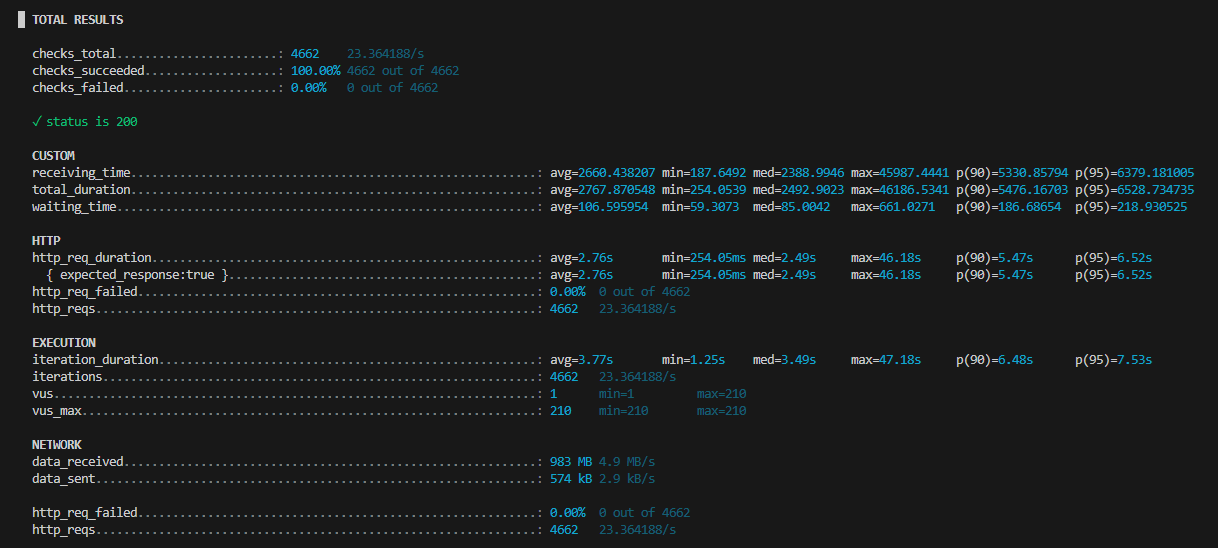
\includegraphics[width=0.5\textwidth]{../images/no-compress_exp1_k6screen.png}
\caption{Рисунок 24}
\end{figure}

Результаты с сжатием (gzip 9):
\begin{figure}[h!]
\centering
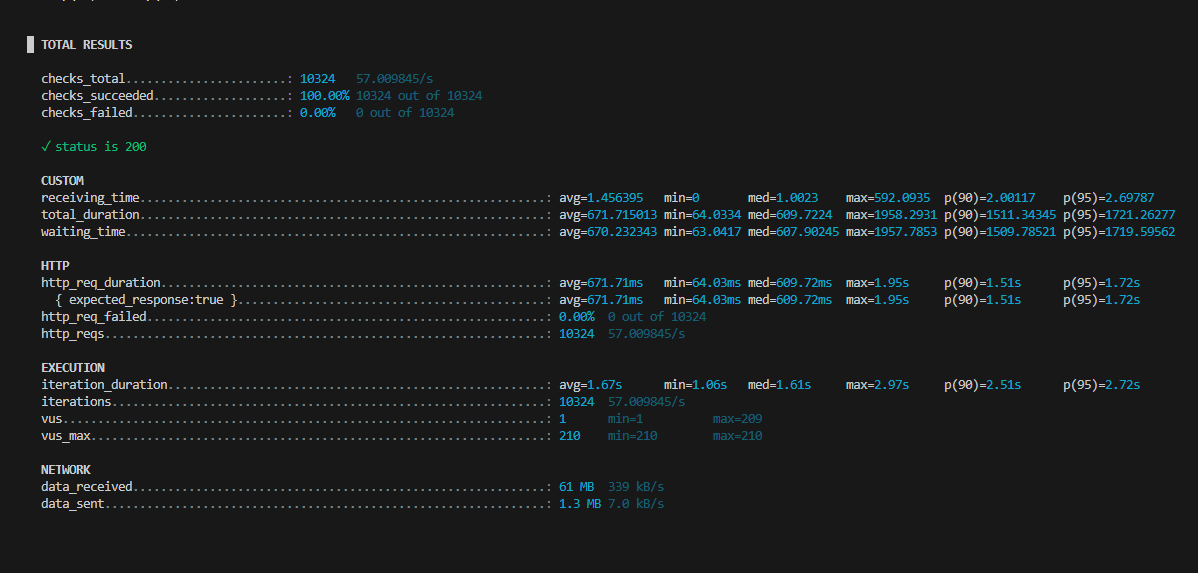
\includegraphics[width=0.5\textwidth]{../images/gzip9_exp1_k6screen.png}
\caption{Рисунок 25}
\end{figure}

Эксперимент второй
Нагрузка:
  stages: [
    { duration: "10s", target: 10 },
    { duration: "20s", target: 10 },
    { duration: "20s", target: 15 },
    { duration: "20s", target: 20 },
    { duration: "20s", target: 25 },
    { duration: "20s", target: 30 },
    { duration: "10s", target: 5 },
  ]

Результаты без сжатия:
\begin{figure}[h!]
\centering
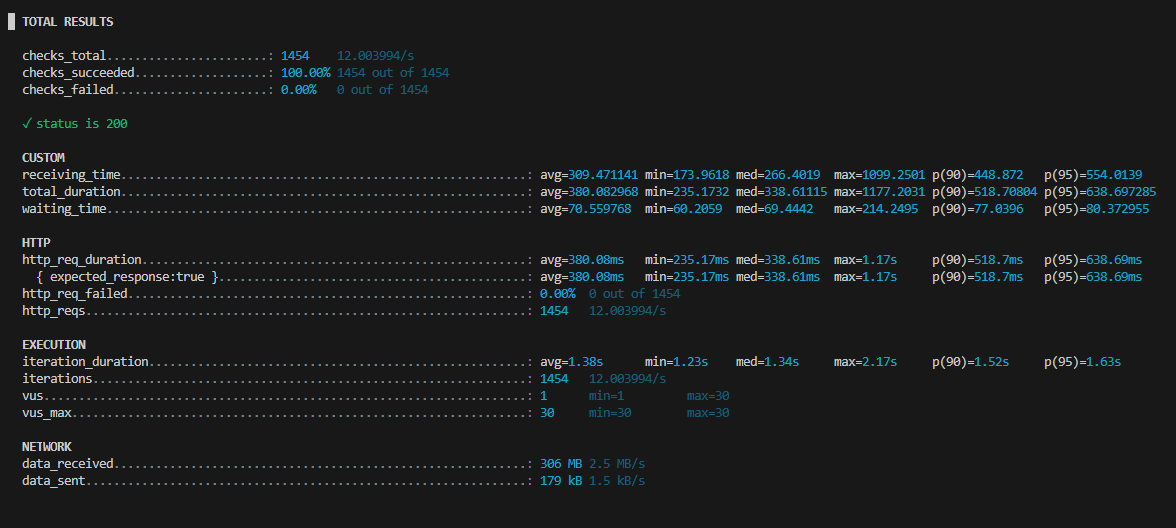
\includegraphics[width=0.5\textwidth]{../images/no-compress_exp2_k6screen.png}
\caption{Рисунок 26}
\end{figure}

Результаты с сжатием (gzip 9):
\begin{figure}[h!]
\centering
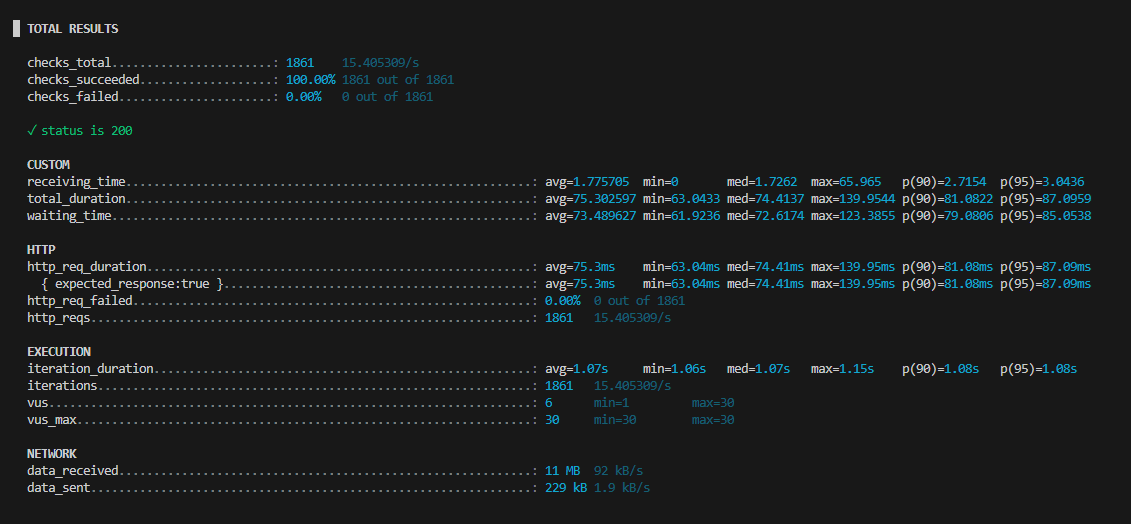
\includegraphics[width=0.5\textwidth]{../images/gzip9_exp2_k6screen.png}
\caption{Рисунок 27}
\end{figure}

Анализ полученных результатов
В первом эксперименте с пиковой нагрузкой прирост в количестве обработанных запросов составил 121%, во втором - 28%.
Заметим, что с ростом числа пользователей, несмотря на чудовищные по меркам сайтов $T{req}=2,6$c, сервер не отклоняет запросы, а ставит их в очередь. Максимальная длина очереди - число пользователей. Пусть $V{max}$ - максильное число запросов, которое сервер может обработать в секунду. Найдём $T_{req}$ в установившемся пиковом режиме. Условие установившегося режима - количество поступающих запросов совпадает с количеством обработанных: 
$\frac{N{users}}{T{req} + T{wait}}=V{max}$
$T{req} = \frac{N{users}}{V{max}} - T{wait}$
Из этой формулы можно найти максимальное число пользователей, при котором начнут отклоняться http запросы: 
$N^{крит}{users} = (T^{крит}{req} + T{wait}){V{max}}$
Так, для $T^{крит}{req} = 10$с, $T{wait}=1$c, $V{max}=80$RPS, $N^{крит}{users}=880$
В первом эксперименте обе конфигурации вышли на пиковый режим. В случае без сжатия узким горлышком оказалась сеть, во втором - мощность процессора. 
Зависимость CPU load, Network load от уровня сжатия (Без переключателя)
Ограничение на скорость создано искусственно с помощью настройки роутера QoS, максимальная скорость около 200 Mb/s
Ограничие скорости гарантирует постоянную полосу пропускания
На сервере отключены все построронние процессы. CPU используется только для:

MySQL Database
Backend server (Express.js)
Обратный прокси сервер (Nginx)

Нагрузка создана с помощью k6:
  stages: [
    { duration: "5s", target: 10 },
    { duration: "10s", target: 20 },
    { duration: "10s", target: 30 },
    { duration: "10s", target: 40 },
    { duration: "10s", target: 50 },
    { duration: "10s", target: 60 },
    { duration: "10s", target: 70 },
    { duration: "10s", target: 80 },
    { duration: "10s", target: 90 },
    { duration: "10s", target: 100 },
    { duration: "10s", target: 110 },
    { duration: "10s", target: 120 },
    { duration: "10s", target: 130 },
    { duration: "10s", target: 140 },
    { duration: "10s", target: 150 },
    { duration: "10s", target: 170 },
    { duration: "10s", target: 190 },
    { duration: "10s", target: 210 },
    { duration: "5s", target: 5 },
  ]

В базе данных находится 400 видео, для тестирования используется Get запрос:
/video/getRecomendations/1, который возвращает 100 случайных видео из базы данных. Около 100 видео, нужно для реализации корректного
скроллинга. (В одной строке можно разместить 5 видео, На экране помещается 5 строк, хотим закрыть
потребность в 3 скролах без подзагрузки, получаем 100 видео). 
Будет варироваться степень сжатия:

no compress
gzip 1
gzip 5
gzip 9

При построении графиков использовалось сглаживание по трём точкам
$x^{smooth}{i} = \frac{x{i-1} + x{i} + x{i+1}}{3}$
Построены графики от времени
Результаты измерений
No compress
\begin{figure}[h!]
\centering
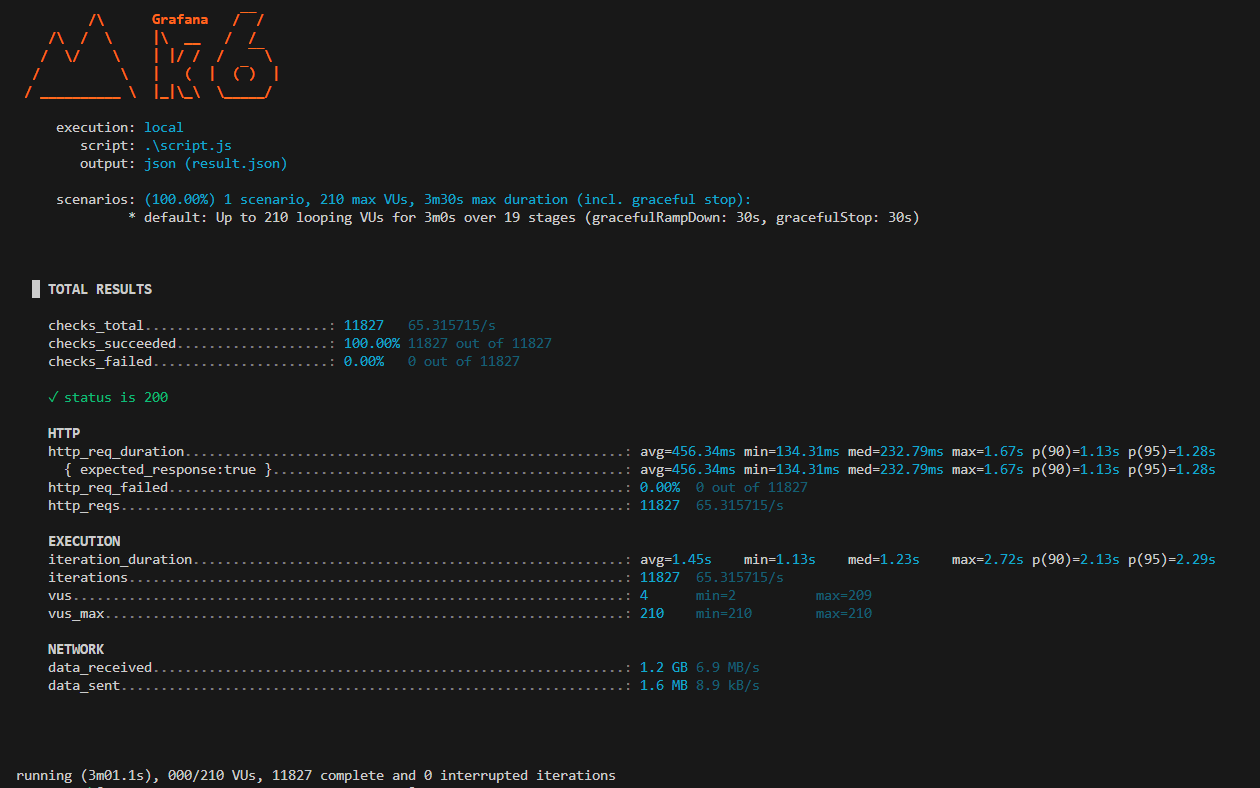
\includegraphics[width=0.5\textwidth]{../images/second_part/no_compress_screenshot.png}
\caption{Рисунок 28}
\end{figure}

Gzip level 1
\begin{figure}[h!]
\centering
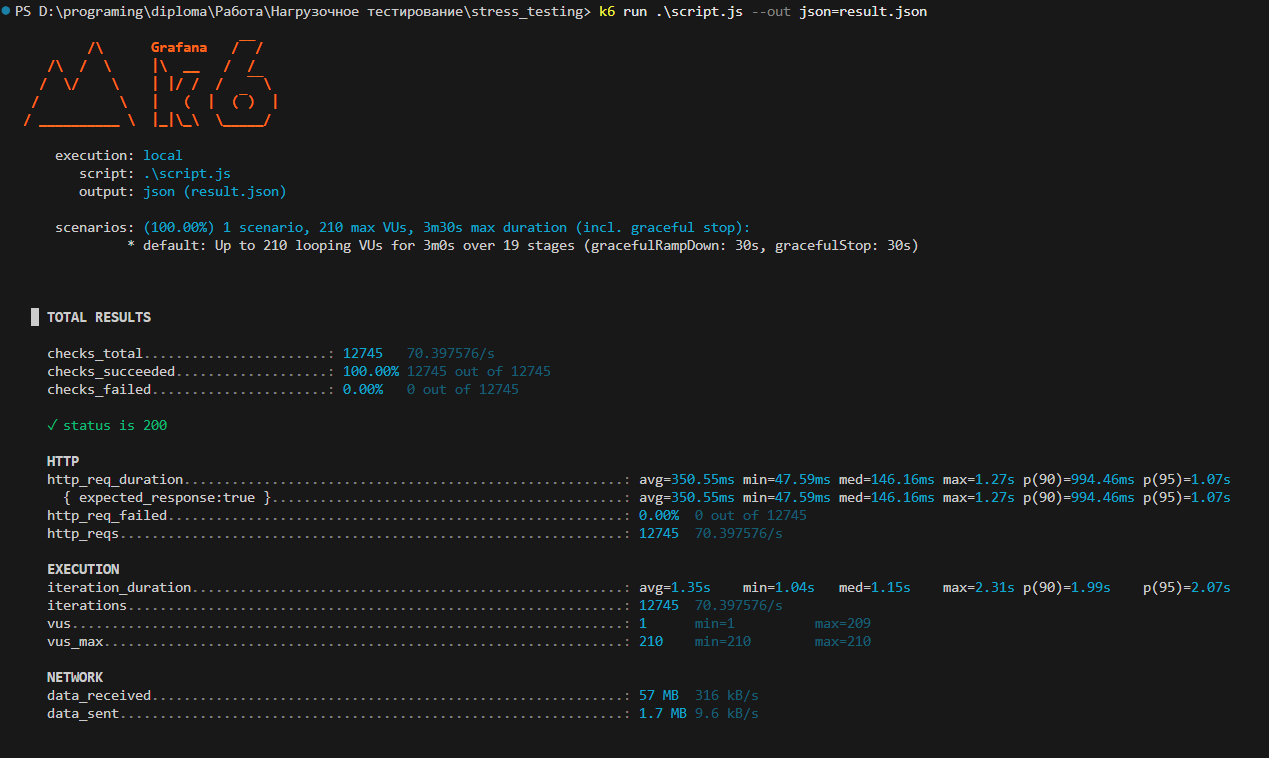
\includegraphics[width=0.5\textwidth]{../images/second_part/gzip1_screenshot.png}
\caption{Рисунок 29}
\end{figure}

Gzip level 5
\begin{figure}[h!]
\centering
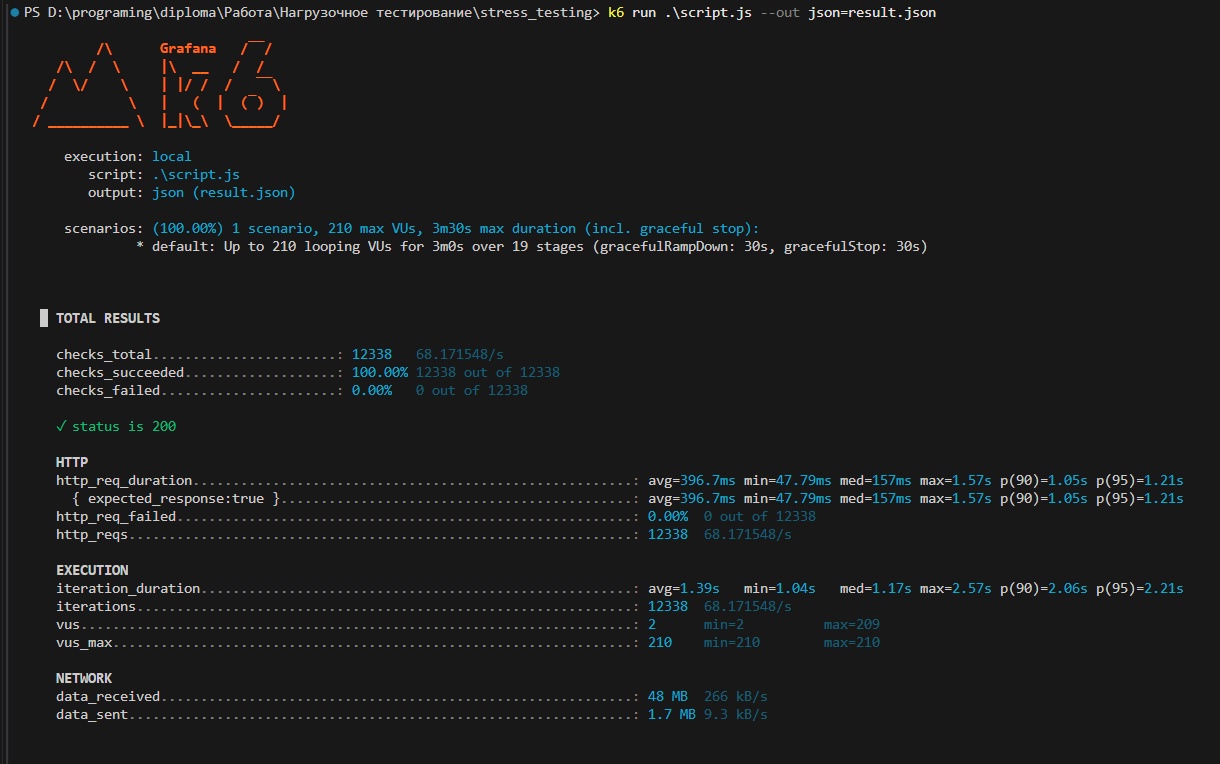
\includegraphics[width=0.5\textwidth]{../images/second_part/gzip5_screenshot.png}
\caption{Рисунок 30}
\end{figure}

Gzip level 9
\begin{figure}[h!]
\centering
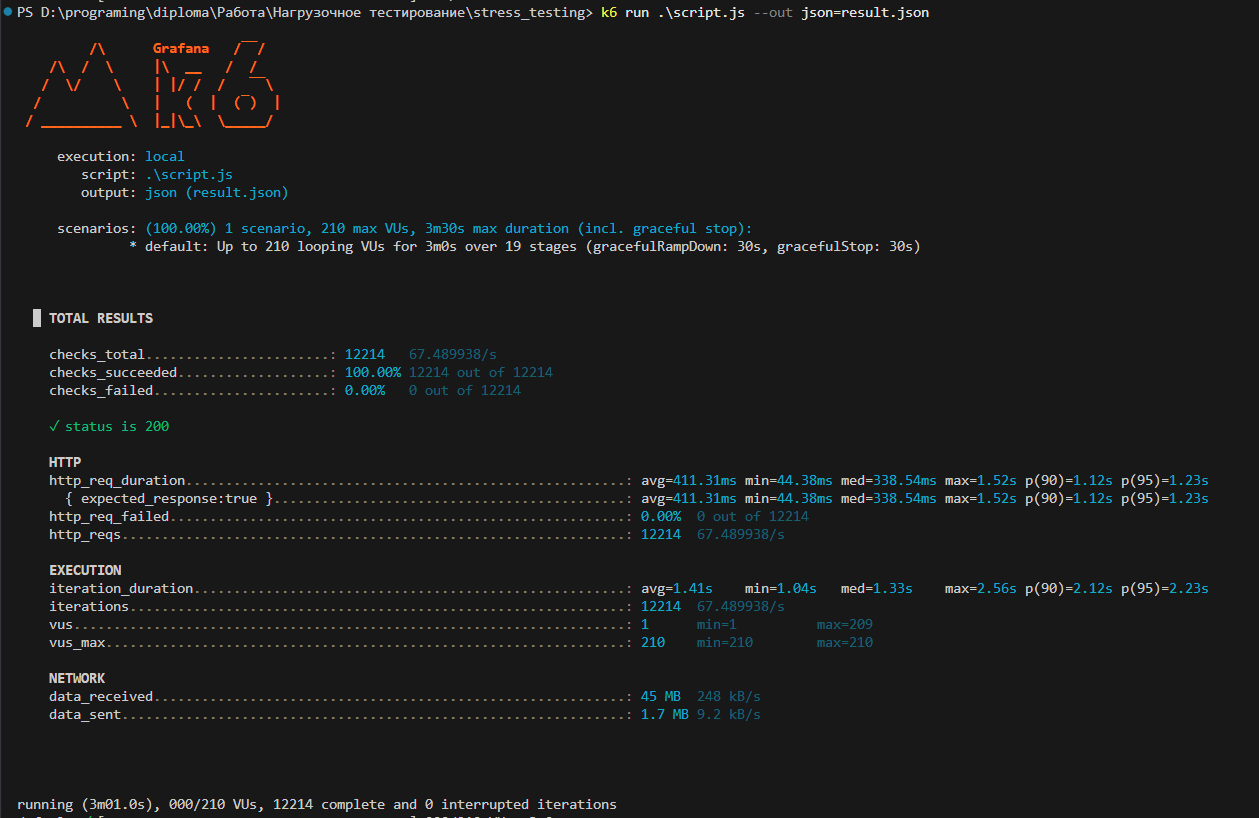
\includegraphics[width=0.5\textwidth]{../images/second_part/gzip9_screenshot.png}
\caption{Рисунок 31}
\end{figure}

Requests per seconds
\begin{figure}[h!]
\centering
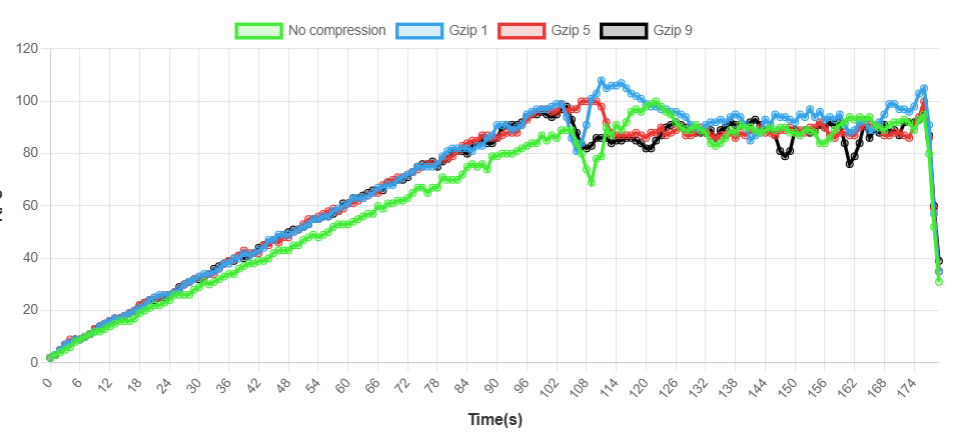
\includegraphics[width=0.5\textwidth]{../images/second_part/RPS.png}
\caption{Рисунок 32}
\end{figure}

Cpu load
\begin{figure}[h!]
\centering
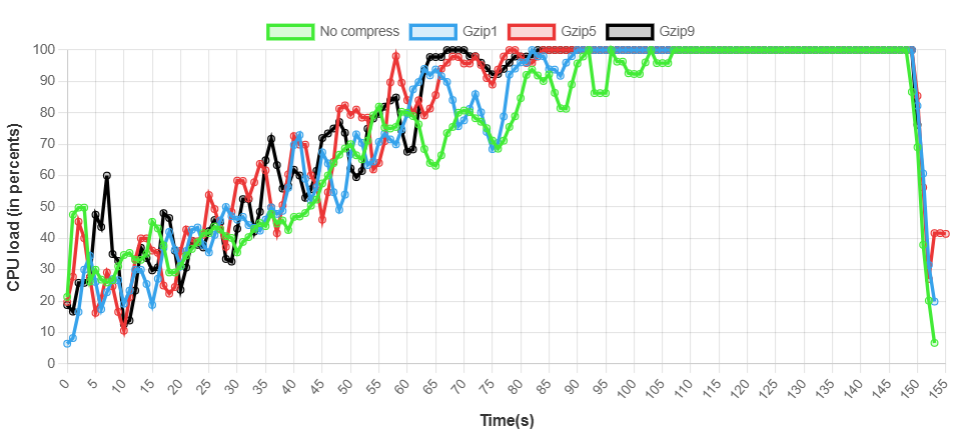
\includegraphics[width=0.5\textwidth]{../images/second_part/CPU_load.png}
\caption{Рисунок 33}
\end{figure}

Transmission speed
\begin{figure}[h!]
\centering
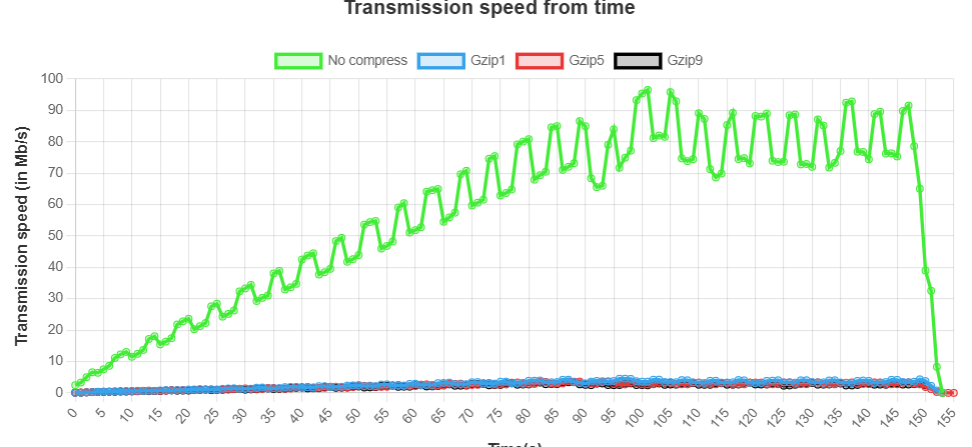
\includegraphics[width=0.5\textwidth]{../images/second_part/Transmission_speed.png}
\caption{Рисунок 34}
\end{figure}

\begin{figure}[h!]
\centering
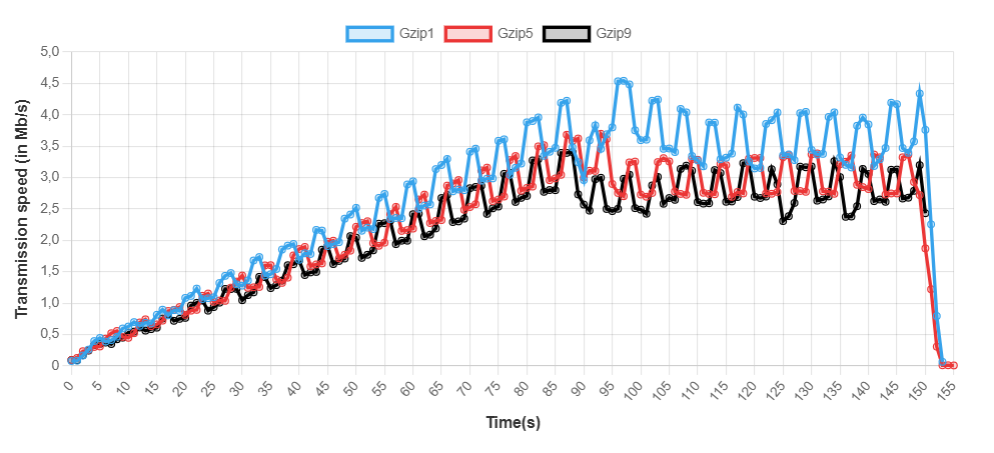
\includegraphics[width=0.5\textwidth]{../images/second_part/Transmission_speed_withot_nocompress.png}
\caption{Рисунок 35}
\end{figure}

Анализ полученных результатов
Как видно, использовние gzip заментно снизило нагрузку на сеть примерно в 20-30 раз,
при этом даже при 80 МБ/c несжатого трафика, нагрузка на CPU из-за сжатия оказалась крайне малой, что при загрузке CPU на 100%,
показатель RPS остался на том же уровне.
3.5 Реализация переключателя
Чтобы реализовать переключатель степени сжатия, используя указанный стек технологий, можно использовать один из 3-х способов: 
Дополнительный обратный прокси сервер на Express.js
При первой попытке создания переключателя стало понятно, что стандартная реализация библиотеки Gzip и в целом Nginx не поддерживают динамическое изменение степени сжатия для конкретного HTTP запроса. То есть в Nginx можно прописать разное сжатие по адресам, это выглядит примерно так:
http 
    gzip on;
    gzip_types application/json text/plain text/css application/javascript application/xml;
    gzip_min_length 100;
    gzip_vary on;
    include /etc/nginx/conf.d/*.conf;

    server 
        listen 3002;
        add_header Vary Accept-Encoding;

        location ^~ /gzip/1/ {
            gzip_comp_level 1;
            rewrite ^/gzip/1/(.*)$ /$1 break;
            proxy_pass http://server:3001;
        }

        location ^~ /gzip/2/ {
            gzip_comp_level 2;
            rewrite ^/gzip/2/(.*)$ /$1 break;
            proxy_pass http://server:3001;
        }
    ...

То есть для адреса /gzip/1/* применяем сжатие gzip 1, для адреса /gzip/2/* применем сжатие gzip 2 и т.д. Но браузер сам не будет получать информацию о загрузке сети и процессора сервера и перенаправлять запросы. Для этой задачи я использовал ещё один обратный прокси сервер на Express js, который проверял с заданным промежутком загрузку процессора и перенаправлял запрос /someadress/ на /gzip/n/someadress. 
К сожалению, затраты на создание ещё одного прокси оказались слишком велики, при любой конфигурации сети, количество обработанных запросов такого переключателя было более чем на 10% меньше чем статическое сжатие с помощью Nginx gzip 1.
Реконфигуратор Nginx
Существует команда nginx -s reload, которая выполняет безопасную перезагрузку конфигурационного файла
Получив сигнал, главный процесс проверяет правильность синтаксиса нового конфигурационного файла и пытается применить содержащуюся в нём конфигурацию:
- Если это удаётся, главный процесс запускает новые рабочие процессы и отправляет сообщения старым рабочим процессам с требованием завершиться.
- В противном случае главный процесс откатывает изменения и продолжает работать со старой конфигурацией.  
Старые рабочие процессы, получив команду завершиться, прекращают принимать новые запросы и продолжают обслуживать текущие запросы, пока все такие запросы не будут обслужены. После этого старые рабочие процессы завершаются.  
Таким образом, эта команда позволяет в реальном времени без опасения потерять необработанные запросы сменить конфигурационный файл. Я создал 10 конфигурационных файлов: 1 без сжатия, 9 - для каждого уровня gzip. И с помощью дополнительной программы менял их и перезагружал Nginx
Модуль для Nginx
Для Nginx можно написать свой модуль, который будет выполнять роль переключателя. В ходе данной работы я его не реализовал 
4. Вывод (практически показать, что реально сделано)
Приложение
Типы файлов в браузере
Каждый раз, когда браузер получает файл с веб-сервера, сервер добавляет заголовок “Content Type” этому файлу. Ваш браузер соотносит “Content Type” со списком его собственных “MINE Types”, чтобы понять, что дальше делать с этим конкретным файлом.
Например, чтобы отобразить PNG изображение на сайте, файл с изображением должен иметь “Content Type” “image/png”, когда браузер его скачивает. Это даёт понимание браузеру, что он получил необходимый файл и может попробовать отобразить его на экране.
MIME расшифровывается как "Multipurpose Internet Mail Extensions". Концепция MINE Types” была изначально придумана для использования в электронной почте, поэтому “Mail” присутствует в аббревиатуре. Сейчас “Mine Types” так же используются в веб-приложениях.
Браузеры поддерживают широкий спектр MIME-типов. Вот некоторые из наиболее распространенных MIME-типов, которые поддерживаются современными браузерами:
Текстовые данные

text/html: HTML-документы
text/css: Таблицы стилей CSS
text/javascript или application/javascript: JavaScript-файлы
text/plain: Обычные текстовые файлы

Изображения

image/jpeg: JPEG-изображения
image/png: PNG-изображения
image/gif: GIF-изображения
image/webp: WebP-изображения
image/avif: AVIF - изображения
image/svg+xml: SVG векторная графика

Аудио и видео

audio/mpeg: MP3 аудио
audio/ogg: OGG аудио
audio/wav: WAV аудио
video/mp4: MP4 видео
video/webm: WebM видео
video/ogg: Ogg видео

Документы

application/pdf: PDF файлы
application/xml: XML файлы
application/json: JSON данные

Приложения

application/octet-stream: Для необработанных двоичных файлов
application/zip: ZIP архивы

Шрифты

font/woff: WOFF шрифты
font/woff2: WOFF2 шрифты
application/vnd.ms-fontobject: EOT шрифты
font/ttf: TTF шрифты

\end{document}